\documentclass{article}

% If your paper is accepted, change the options for the package
% aistats2020 as follows:
%
% \usepackage[accepted]{aistats2020}
%
% This option will print headings for the title of your paper and
% headings for the authors names, plus a copyright note at the end of
% the first column of the first page.

% If you set papersize explicitly, activate the following three lines:
%\special{papersize = 8.5in, 11in}
%\setlength{\pdfpageheight}{11in}
%\setlength{\pdfpagewidth}{8.5in}

% If you use natbib package, activate the following three lines:
\usepackage[round]{natbib}
\renewcommand{\bibname}{References}
\renewcommand{\bibsection}{\subsubsection*{\bibname}}

% If you use BibTeX in apalike style, activate the following line:
%\bibliographystyle{apalike}

\usepackage[T1]{fontenc}    % use 8-bit T1 fonts
\usepackage{hyperref}       % hyperlinks
\usepackage{url}            % simple URL typesetting
\usepackage{booktabs}       % professional-quality tables
\usepackage{amsfonts}       % blackboard math symbols
\usepackage{nicefrac}       % compact symbols for 1/2, etc.
\usepackage{microtype}      % microtypography

% My packages

\usepackage[mathscr]{euscript}
\usepackage{graphicx}
\usepackage {tikz}
\usetikzlibrary {positioning}
\usetikzlibrary{shapes.misc}
\usetikzlibrary{shapes.geometric}
\usetikzlibrary{calc}
\usetikzlibrary{arrows.meta}
\usetikzlibrary{intersections}
\usepackage{amsthm}
\usepackage{amsmath}
\usepackage{amssymb}
\usepackage{dsfont}
\usepackage{stmaryrd }
\usepackage{csquotes}
\usepackage{wasysym}
\usepackage[]{todonotes}
\usepackage[shortlabels]{enumitem}
\usepackage{bm}
\usepackage{isomath}
\usepackage{mathtools}

\makeatletter
\newcommand{\newreptheorem}[2]
  {\newtheorem*{rep@#1}{\rep@title}\newenvironment{rep#1}[1]
  {\def\rep@title{#2 \ref*{##1}}\begin{rep@#1}}{\end{rep@#1}}}
\makeatother

\theoremstyle{plain}
\newtheorem{theorem}{Theorem}[section]
\newtheorem{corollary}[theorem]{Corollary}
\newtheorem{lemma}[theorem]{Lemma}
\newtheorem{proposition}[theorem]{Proposition}
\newreptheorem{theorem}{Theorem}

\newtheorem{innercustomthm}{Theorem}
\newenvironment{customthm}[1]
  {\renewcommand\theinnercustomthm{#1}\innercustomthm}
  {\endinnercustomthm}

\theoremstyle{definition}
\newtheorem{definition}[theorem]{Definition}
\newtheorem{example}[theorem]{Example}

\DeclareMathAlphabet{\mathsfit}{T1}{\sfdefault}{\mddefault}{\sldefault}

\newcommand{\CI}{\mathrel{\text{\scalebox{1.07}{$\perp\mkern-10mu\perp$}}}}
\newcommand{\CII}{\mathrel{\text{\scalebox{1.07}{$\perp\mkern-10mu\perp\mkern-10mu\perp$}}}}
\newcommand{\RV}[1]{\ensuremath{\mathsf{#1}}}
\newcommand{\URV}[1]{\ensuremath{\underline{\RV{#1}}}}
\newcommand{\PA}[2]{\ensuremath{\text{Pa}_{#1}(#2)}}
\newcommand{\ND}[2]{\ensuremath{\text{ND}_{#1}(#2)}}
\newcommand{\CH}[2]{\ensuremath{\text{Ch}_{#1}(#2)}}
\newcommand{\DE}[2]{\ensuremath{\text{De}_{#1}(#2)}}
\newcommand{\ID}[1]{\ensuremath{\text{Id}_{#1}}}
\newcommand{\utimes}{\ensuremath{\underline{\otimes}}}
\newcommand{\prob}[1]{\ensuremath{\mathbb{#1}}}
\newcommand{\kernel}[1]{\ensuremath{\mathbf{#1}}}
\newcommand{\model}[1]{\ensuremath{\mathbb{#1}}}
\newcommand{\seedo}{\ensuremath{\mathbb{T}}}
\newcommand{\diagram}[1]{\ensuremath{\mathscr{#1}}}
\newcommand{\sigalg}[1]{\ensuremath{\mathcal{#1}}}
\newcommand{\vecRV}[1]{\ensuremath{\mathsfbfit{#1}}}
\newcommand{\vecVal}[1]{\ensuremath{\mathbf{#1}}}
\newcommand{\prodSet}[1]{\ensuremath{\mathbf{#1}}}
\newcommand{\indx}[1]{\ensuremath{\mathcal{#1}}}
\newcommand{\nod}[1]{\ensuremath{\mathsfit{#1}}}

\makeatletter
\newcommand*\bigcdot{\mathpalette\bigcdot@{.5}}
\newcommand*\bigcdot@[2]{\mathbin{\vcenter{\hbox{\scalebox{#2}{$\m@th#1\bullet$}}}}}
\makeatother

\tikzset{
    triangle/.style = {regular polygon, regular polygon sides=3 },
    node rotated/.style = {rotate=90},
    border rotated/.style = {shape border rotate=90},
    dist/.style = {triangle,draw,border rotated, inner sep=0pt},
    smalldist/.style = {triangle,draw,border rotated},
    kernel/.style={rectangle,draw,inner sep = 2pt},
    expectation/.style = {triangle,draw,inner sep=0pt,shape border rotate=270},
    copymap/.style = {circle,fill,inner sep=1pt}}

\newcommand\DCI{
    \begin{tikzpicture}[scale=0.35]
    \draw[->] (1,0) -- (0,0);
    \draw (0.6,0) -- (0.6,0.75);
    \draw (0.4,0) -- (0.4,0.75);
    \end{tikzpicture}
}

\newcommand\splitter[1]{%
\begin{tikzpicture}[scale=#1]
\draw (0,-1) -- (0,0);
\draw (0,0) to [bend right] (1,1);
\draw (0,0) to [bend left] (-1,1);
\end{tikzpicture}
}

\newcommand\stopper[1]{%
\begin{tikzpicture}[scale=#1]
\draw[-{Rays [n=8]}] (0,-1) -- (0,0);
\end{tikzpicture}
}

\newcommand\source[1]{%
\begin{tikzpicture}[scale=#1]
\path (0,0) node[prob,fill=gray] (P) {};
\draw (P) -- ($(P.east) + (1,0)$);
\end{tikzpicture}
}

\DeclareMathOperator*{\argmax}{arg\,max}
\DeclareMathOperator*{\argmin}{arg\,min}
\DeclareMathOperator*{\arginf}{arg\,inf}
\DeclareMathOperator*{\argsup}{arg\,sup}

\newcommand{\cheng}[1]{ {\color{purple}[{\bf Cheng:~{#1}}]} }

\title{Modular probability for causal modelling}
\date{\today}

\author{ David Johnston }

\begin{document}

\maketitle


% \begin{abstract}

\section{Introduction}

The typical way to construct a probability model is to define a sample space $(\Omega,\sigalg{F})$ and an ambient probability measure $\prob{P}:\sigalg{F}\to[0,1]$, which together form a ``probability space'' $(\prob{P},\Omega,\sigalg{F})$. Random variables are then defined as measurable functions on the sample space $\RV{X}:(\Omega,\sigalg{F})\to (Q,\sigalg{Q})$. Under this theory, the names given to random variables are arbitrary. However, in practice the names given to random variables are not arbitrary: it is fairly common to talk about two different probability distributions $\prob{P}_1[\RV{X}]$ and $\prob{P}_2[\RV{X}]$ over the same random variable with the intention that these define two different models of the same set of propositions. Alternatively, we might define two probability spaces $(\prob{P}_1,\Omega,\sigalg{F})$, $(\prob{P}_2,\Omega,\sigalg{F})$ on the same sample space with random variables $\RV{X}:\Omega\to A$ and $\RV{Y}:\Omega\to A$ given by the same measurable functions $\RV{X}(\omega)=\RV{Y}(\omega)$ but with the intention that $\prob{P}_1(\RV{X})$ and $\prob{P}_2(\RV{Y})$ model different phenomena. Such issues are particularly prevalent in causal modelling, where (for example) we might take a probability distribution $\prob{P}[\RV{X}\RV{Y}\RV{Z}]$, then modify it in accordance with the do-calculus with respect to some graph $\mathcal{G}$ to obtain $\prob{P}[\RV{Y}|do(\RV{X}=x)]$. Clearly $\prob{P}[\RV{X}\RV{Y}\RV{Z}]$ and $\prob{P}[\RV{Y}|do(\RV{X}=x)]$ are different probability distributions, and the variable $\RV{Y}$ seems to refer to the same set of propositions in each. 

Here we propose a theory of variable naming that formally specifies a method for dealing with ``variable names''. We define \emph{named variables} as a subset of random variables -- namely, those random variables that we care to give names. A \emph{modelling context} holds a number of different conditional probability spaces along with a collection of named random variables. Random variables names function similarly to type definitions -- the conditional probability distributions in each probability space can be combined in an operation that we call \emph{extension} with arbitrary conditional probabilities providing that the names of their respective named variable sets can be matched in appropriate ways. We call this ``modular probability'', as it enables us to take collections of conditional probabilities from our modelling context and assemble them like lego pieces, if they have the right attachments for one another.

Our contributions are:

\begin{itemize}
  \item A theory of named variables
  \item Using this theory, we explore causal models under the decision theoretic, graphical model and potential outcomes approach, and show how the latter two approaches can be embedded in the former approach
  \item We examine an ambiguity in the definition of Causal Bayesian Networks that is made obvious when we attempt to apply our theory of named varibles
  \item We examine how a particular kind of lego piece -- a \emph{comb} -- arises repeatedly in causal models and gives a natural way to understand conditional vs ``causal'' dependece
\end{itemize}


% \end{abstract}
\tableofcontents


%!TEX root = main.tex


\section{Variables and Probability Models}\label{sec:vague_variables}

\subsection{Semantics of observed and unobserved variables}\label{sec:variables}

We are interested in constructing \emph{probabilistic models} which explain some part of the world. In a model, variables play the role of ``pointing to the parts of the world the model is explaining''. Both observed an unobserved variables play important roles in causal modelling and we think it is worth clarifying what variables of either type refer to. Ultimately, our interpretation is largely the standard one: a probabilistic model is associated with an experiment or measurement procedure that yields values in a well-defined set. Observable variables are obtained by applying well-defined functions to the result of this total measurement. We explain how we can use a richer sample space that includes unobserved variables. Unobserved variables are formally modelled in exactly the same way as observed variables, but unlike observed variables we don't offer a standard interpretation of unobserved variables. 

Consider Newton's second law in the form $\proc{F}=\proc{MA}$ as a simple example of a model that relates variables $\proc{F}$, $\proc{M}$ and $\proc{A}$. As \citet{feynman_feynman_1979} noted, this law is incomplete -- in order to understand it, we must bring some pre-existing understanding of force, mass and acceleration as independent things. Furthermore, the nature of this knowledge is somewhat perculiar. Acknowledging that physicists happen to know a great deal about determining the forces on an object, it remains true that in order to actually say what the net force on a real object is, even a highly knowledgeable physicist will still have to go and do some measurements, and the result of such measurements will be a vector representing the net forces on that object.

This suggests that we can think about ``force'' $\proc{F}$ (or mass or acceleration) as a kind of procedure that we apply to a particular real world object and which returns a mathematical object (in this case, a vector). We will call $\proc{F}$ a \emph{procedure}. Our view of $\proc{F}$ is akin to \citet{menger_random_2003}'s notion of variables as ``consistent classes of quantities'' that consist of pairing between real-world objects and quantities of some type. Force $\proc{F}$ itself is not a well-defined mathematical thing, as measurement procedures are not mathematically well-defined. At the same time, the set of values it can return \emph{are} well-defined mathematical things. 

The fact that procedures return well-defined mathematical quantities allows us to define an operation akin to function composition. If I have a procedure $\proc{B}$ that takes values in some set $B$, and a function $f:B\to C$, define the ``composition'' $f\circ \proc{B}$ to be the procedure given by applying the procedure $\proc{B}$ and then applying $f$ to the result. For example, $\proc{MA}$ is the composition of $h:(x,y)\mapsto xy$ with $(\proc{M},\proc{A})$ that measures the mass and acceleration of the same object, and returns their values in an ordered pair.

One might whether there is also some kind of ``append'' operation that takes a standalone $\proc{M}$ and a standalone $\proc{A}$ and returns a procedure $(\proc{M},\proc{A})$. Unlike function composition, this would be an operation that acts on two procedures rather than a procedure and a function. Rather than attempt to define any operation of this type, we simply assume that somehow a procedure has been devised that measures everything of interest, which we will call $\proc{S}$ which takes values in $\Psi$. We assume $\proc{S}$ is such that any procedure of interest can be written as $f\circ \proc{S}$ for some $f$.

For the model $\proc{F}=\proc{MA}$, for example, we could assume $\proc{F}=f\circ \proc{S}$ for some $f$ and $(\proc{M},\proc{A})=g\circ \proc{S}$ for some $g$. In this case, we can get $\proc{MA}=h\circ(\proc{M},\proc{A})=(h\circ g)\circ\proc{S}$. Note that each procedure is associated with a unique function with domain $\Psi$.

Thus far, $\Psi$ is a ``sample space'' that only contains observable variables. To include unobserved variables, we posit a richer sample space $\Omega$ such that the measurement $\proc{S}$ determines an element of some partition of $\Omega$ rather than an element of $\Omega$ itself. Then, by analogy to procedures defined with respect to $\proc{S}$, we identify variables in general with measurable functions defined on the domain $\Omega$. 

Specifically, suppose $\proc{S}$ takes values in $\Psi$. Then we can propose a sample space $\Omega$ such that $|\Omega|\geq |\Psi|$ and a surjective function $\RV{S}:\Omega\to \Psi$ associated with $\proc{S}$. We connect $\Omega$, $\RV{S}$ and $\proc{S}$ with the notion of \emph{compatibility with obseravation}:

\begin{align}
 &\omega\in \Omega\text{ is \emph{compatible with observation} iff the result yielded by }S\text{ is equal to }\RV{S}(\omega)\label{def:observable}
\end{align}

Thus the procedure $\proc{S}$ eventually restricts the observationally compatible elements of $\Omega$ to some subset induced by $\RV{S}$; we may or may not add additional postulates to choose from the remaining candidates. A probability model on $\Omega$ could be regarded as a forecast of which elements of $\Omega$ are likely to be observationally compatible. If we have a formal variable $\RV{X}$ that can be written as $f\circ \RV{S}$ for some $f$, then $\RV{X}$ is an \emph{observed variable}, otherwise it is an \emph{unobserved variable}.

One thing to note in this setup is that two different sets of measurement outcomes $\Psi$ and $\Psi'$ entails specifying an different mesurement procedurees $\proc{S}$ and $\proc{S}'$. On the other hand, it is possible to define different sample spaces $\Omega$ and $\Omega'$ that share a single procedure $\proc{S}$ (recall that the procedure $\proc{S}$ does not itself depend on $\Omega$, though its model $\RV{S}$ does). We will sometimes consider different models of the same observable procedurees.

As far as we know, distinguishing variables from procedurees is somewhat nonstandard, but it is useful because, as we have discussed, every procedure is assumed to be modeled by a variable but not every variable is a model of a procedure. Furthermore, while they may not be distinguished, both variables and procedurees are often discussed in statistical texts. For example, \citet{pearl_causality:_2009} offers the following two, purportedly equivalent, definitions of variables:
\begin{quote}
By a \emph{variable} we will mean an attribute, measurement or inquiry that may take on one of several possible outcomes, or values, from a specified domain. If we have beliefs (i.e., probabilities) attached to the possible values that a variable may attain, we will call that variable a random variable.
\end{quote}

\begin{quote}
This is a minor generalization of the textbook definition, according to which a random variable is a mapping from the sample space (e.g., the set of elementary events) to the real line. In our definition, the mapping is from the sample space to any set of objects called ``values,'' which may or may not be ordered.
\end{quote}

Variables model procedurees, but they are not the same thing as procedurees.

\subsection{Events}

To recap, we have a procedure $\proc{S}$ yielding values in $\Psi$ that measures everything we are interested in, a sample space $\Omega$ and a function $\RV{S}$ that models $\proc{S}$ in the sense of Definition \ref{def:observable}. We assume also that $\Psi$ has a $\sigma$-algebra $\sigalg{E}$ (this may be the power set of $\Psi$, as measurement procedurees are typically limited to finite precision). $\Omega$ is equipped with a $\sigma$-algebra $\sigalg{F}$ such that $\sigma(\RV{S})\subset \sigalg{F}$. If a procedure $\proc{X}=f\circ \RV{S}$ then we define $\RV{X}:\Omega\to X$ by $\RV{X}:=f\circ\RV{S}$.

If a particular procedure $\proc{X}=f\circ \proc{S}$ eventually yields a value $x$, then the values of $\Omega$ compatible with observation are a subset of $\RV{X}^{-1}(x)$. We define $\RV{X}\bowtie x:\cong \RV{X}^{-1}(x)$, which we read ``$\RV{X}$ yields x''. This definition applies to all types of variables, not just observables, but we only provide an interpretation of the meaning of this definition when $\RV{X}$ is associated with $\proc{X}$: in that case, $\RV{X}\bowtie x$ contains the compatible values of $\Omega$ iff $\proc{X}$ yields x. 

We extend this to say, for measurable $A\in \sigalg{X}$, $\RV{X}\bowtie A=\bigcup_{x\in A} \RV{X}\bowtie x$. Given $\RV{Y}:\Omega\to X$, $\RV{X}\bowtie \RV{Y}=\bigcup_{x\in X} \RV{X}\bowtie x \cap \RV{Y}\bowtie x$, read ``$\RV{X}$ yields the same as $\RV{Y}$''. $\RV{X}\not\bowtie x:\cong (\RV{X}\bowtie x)^C$.

We use a bowtie to stand for ``yields'': $\RV{Y}\bowtie y :\cong \RV{Y}^{-1}(y)$. It is somewhat common to use the symbol ``$=$'' to do this job, but we do not want to do this because $\RV{Y}=y$ already has a meaning, namely that $\RV{Y}$ is a constant function everywhere equal to $y$. 

\subsection{Probabilistic models}

We've offered an interpretation of variables, but we won't offer a similar interpretation of probability. Interpreting probability is notoriously difficult. Incidentally, conditioning on different values of unobserved variables typically induces different probability models over observed variables, so supplying an interpretion of what it means for a probability model to be ``correct'' might also entail an interpretation of what it means for an unobserved variable to yield a particular value.

We will assume for the time being that we want to construct probabilistic models that relate collection of variables, defined as they have been above. The standard method for 

Throughout this paper, we will assume all measurable sets are finite sets. This is because it makes explanations simpler and because it is easy to show that conditional probabilities exist in this setting (Lemma \ref{lem:subm_exist}).

At this point we have a crude model of some observation procedure $\proc{S}$ given by $\Omega$ and a collection of variables, and we can relate a claim that some $\omega$ is \emph{compatible with observations} to real-world events via the procedure $\proc{S}$. We wish to extend this with probability distributions and conditional probabilties. A probability distribution $\prob{P}^{\RV{X}}$ for some variable $\RV{X}:\Omega\to B$ is a probability measure on $(B,\sigalg{B})$, and a conditional probability $\prob{P}^{\RV{X}|\RV{Y}}$ for $\RV{X}:\Omega\to B$, $\RV{Y}:\Omega\to C$ is a Markov kernel $B\kto C$. A a probability distribution $\mu$ on $(B,\sigalg{B})$ is a $\sigma$-additive measure $\mu:\sigalg{B}\to [0,1]$ such that $\mu(\emptyset)=0$ and $\mu(B)=1$, and a Markov kernel $\kernel{K}:B\kto C$ is a is a map $B\times \sigalg{C}\to [0,1]$ such that

\begin{itemize}
	\item x\mapsto \kernel{K}(x,A) is $\sigalg{B}$-measurable for all $A\in \sigalg{C}$
	\item A\mapsto \kernel{K}(x,A) is a probability measure on $(C,\sigalg{C})$ for all $x\in B$
\end{itemize}

Given $\prob{P}^{\RV{X}}$, we identify $\prob{P}^{\RV{X}}(\{x\})$ with the probability $\prob{P}(\RV{X}\bowtie x)$ of the event $\RV{X}\bowtie x$ under some related probability measure $\prob{P}$ on $(\Omega,\sigalg{F})$. That is, we assume that there exists some $\prob{P}$ on $(\Omega,\sigalg{F})$ such that $\prob{P}^{\RV{X}}(\{x\})=\prob{P}(\RV{X}\bowtie x)$. More generally, we say a collection of probability distributions $\{\prob{P}^{\RV{X}_i}|i\in D\}$ is \emph{sample space compatible} if there exists $\prob{P}$ on $\Omega$ such that $\prob{P}^{\RV{X}_i}(A)=\prob{P}(\RV{X}_i\bowtie A)$ for all $A\in \sigalg{B}$, $i\in D$.

Extending sample space compatibility to conditional probabilities is somewhat trickier, because conditional probably does not seem to have a simple correspondence to any more fundamental notion. See for example \citet{hajek_what_2003} for some difficulties with defining conditional probability purely in terms or a probability measure $\prob{P}$ on $(\Omega,\sigalg{F})$, and \citet{nguyen_probability_2002} for a difficulties with interpreting conditional probability as the probability of an implication.

We say a collection of conditional probabilities $\{\prob{P}^{\RV{X}_i|\RV{X}_j}|i\in D, j\in E\}$ is sample space compatible relative to $\RV{Y}$ if there exists some $\prob{P}^{;\RV{Y}}:Y\kto \Omega$ such that, for all $j\in E$, $i\in D$:

\begin{align}
	\RV{X}_i^{-1}(A)\cap \RV{X}_{j}^{-1}(b) &= \emptyset \implies \prob{P}^{\RV{X}_i|\RV{X}_j}(A|b)=0 &\forall A\in \sigalg{X}_i, b\in X_j \label{eq:ssc_1}\\
	\prob{P}^{;\RV{Y}}((\RV{X}_i,\RV{X}_j)\bowtie A\times B|c) &= \int_A \prob{P}^{\RV{X}_{i}|\RV{X}_j}(B|\RV{X}_j(\omega))\prob{P}^{;\RV{Y}}(d\omega|c) &\forall c\in Y:\prob{P}^{;\RV{Y}}(\RV{X}_j\bowtie A|c)>0 \label{eq:ssc_2}
\end{align}

$\{\prob{P}^{\RV{X}_i|\RV{X}_j}|i\in D, j\in E\}$ is sample space compatible if there is some $\RV{Y}$ such that it is sample space compatible relative to $\RV{Y}$. Note that Equation \ref{eq:ssc_2} is similar to a standard definition of conditional probability, while Equation \ref{eq:ssc_1} is an additional requirement, roughly saying ``the probability of $u$ given $\not u$ is always zero''. 

By convention, a collection of conditional probabilities with the same base letter $\prob{P}^{\RV{X}|\RV{Y}}$, $\prob{P}^{\RV{Z}|\RV{Y}}$ are held to be jointly sample space compatible.

Consider a model obtained from ``truncated factorisation'', an operation that is typical in causal modelling and atypical in probability theory. Suppose we have a causal Bayesian network $(\prob{P}^{\RV{XYZ}},\mathcal{G})$ where $\RV{X}:\Omega\to A$, $\RV{Y}:\Omega\to B$ and $\RV{Z}:\Omega\to C$ are variables, $\prob{P}^{\RV{XYZ}}$ is a probability measure on $A\times B\times C$ that we call ``a probability model of $(\RV{X},\RV{Y},\RV{Z})$'' and $\mathcal{G}$ is a Directed Acyclic Graph whose vertices we identify with $\RV{X}$, $\RV{Y}$ and $\RV{Z}$ that contains the edges $\RV{X}\longrightarrowRHD \RV{Y}$ and $\RV{X}\longleftarrowRHD \RV{Z} \longrightarrowRHD \RV{Y}$. ``Setting $\RV{X}$ to $x$'' is an operation that takes as inputs $\prob{P}^{\RV{XYZ}}$, $\mathcal{G}$ and some $x\in A$ and returns a new probability measure $\prob{P}_x^{\RV{XYZ}}$ on $A\times B\times C$ given by \citep[page ~24]{pearl_causality:_2009}:
\begin{align}
	\prob{P}^{\RV{XYZ}}_{x}(x',y,z)=\prob{P}^{\RV{Y|XZ}}(y|x,z)\prob{P}^{\RV{Z}}(z)\llbracket x=x' \rrbracket\label{eq:truncated_fac}
\end{align}

Equation \ref{eq:truncated_fac} embodies three assumptions about a model of the operation of ``setting $\RV{X}$ to $x$''. First, such a model must assign probability 1 to the proposition that $\RV{X}$ yields $x$. Second, such a model must assign the same marginal probability distribution to $\RV{Z}$ as the input distribution; $\prob{P}^{\RV{Z}}=\prob{P}_{x}^{\RV{Z}}$. Finally, our model must also assign the same conditional probability to $\RV{Y}$ given $\RV{X}$ and $\RV{Z}$; $\prob{P}^{\RV{Y}|\RV{XZ}}=\prob{P}_x^{\RV{Y}|\RV{XZ}}$.

We cannot always find a sensible probability distribution $\prob{P}_x^{\RV{XYZ}}$ that has the required properties. For example, if $\RV{X}$ and $\RV{Z}$ happen to be represented by the same function -- which is to say, the underlying procedurees $X$ and $Z$ both refer to the same measurement of the same thing -- then any model must surely assign probability 1 to the event $\RV{X}\bowtie \RV{Z}$; or equivalently, probability 0 to the event $\RV{X}\not\bowtie \RV{Z}$. However, this cannot be done in accordance with Equation \ref{eq:truncated_fac} for all $x\in A$ if $|A|\geq 2$. This is because for $x\neq x'\in A$, $\prob{P}_x^{\RV{X}}\neq \prob{P}_{x'}^{\RV{X}}$ but $\prob{P}_x^{\RV{Z}}=\prob{P}_{x'}^{\RV{Z}}$.

Thus we have \emph{four} assumptions to satisfy:
\begin{enumerate}
	\item $\prob{P}_x^{\RV{X}}=1$
	\item $\prob{P}^{\RV{Z}}=\prob{P}_{x}^{\RV{Z}}$
	\item $\prob{P}^{\RV{Y}|\RV{XZ}}=\prob{P}_x^{\RV{Y}|\RV{XZ}}$
	\item If $\RV{X}=\RV{Z}$ then $\prob{P}_x(\RV{X}\bowtie \RV{Z})=1$
\end{enumerate}

Crucially, only assumptions 2 and 3 depend on the assumed causal graph $\mathcal{G}$; assumptions 1 and 4 should hold regardless. As we will show, these assumptions are both implied by the assumption that we have some $\prob{Q}^{\RV{XYZ}|\RV{X}}$ that is \emph{sample space compatible} such that $\prob{P}^{\RV{XYZ}}_x(x',y,z) = \prob{Q}^{\RV{XYZ}|\RV{X}}(x',y,z|x)$. Furthermore, as we will show, Equation \ref{eq:ssc_1} implies assumption 1 and Equation \ref{eq:ssc_2} implies assumption 4, and so both requirements are needed.

The example of $\RV{X}=\RV{A}$ might seem absurd. Consider instead $\RV{Z}=(\RV{H},\RV{W})$, representing the height in metres and weight in kilograms of a particular person, and $\RV{X}$ represents their body mass index, which is to say $\RV{X}=\frac{\RV{W}}{\RV{H}^2}$ (not that in both cases we are using ``$=$'', which means these variables are \emph{equal as functions}, not that they \emph{yield the same result with probability 1}, which would involve the symbol ``$\bowtie$''). A causal graph with exactly these variables and arrows analogous to ours appears in \citet{shahar_association_2009}. However, generally there is no $\prob{P}_x^{\RV{XHW}}$ that satisfies both $\RV{X}\bowtie \frac{\RV{W}}{\RV{H}^2}$ with probability 1 and Equation \ref{eq:truncated_fac}. This is true, for example, whenever $\prob{P}^{\RV{X}}$ has support at more than one point.

\subsection{Operating on Markov kernels with string diagrams}
Markov categories are abstract categories that represent models of the flow of information. Operations like Equation \ref{eq:truncated_fac} are expressible as abstract compositions in Markov categories, and may be represented with string diagrams developed for reasoning about objects in the category. Valid proofs using string diagrams correspond to valid theorems in \emph{any} Markov category, though we will limit our attention to the category of finite sets and Markov kernels in this paper. The main drawback of Markov categories is that, as they exist at the moment, they have no notion of ``variables''. More comprehensive introductions to Markov categories can be found in \citet{fritz_synthetic_2020,cho_disintegration_2019}.

Given measurable sets $(X,\sigalg{X})$ and $(Y,\sigalg{Y})$, a Markov kernel or stochastic map is a map $\kernel{K}:X\times \sigalg{Y}\to [0,1]$ such that

\begin{itemize}
	\item The map $x\mapsto \kernel{K}(x,A)$ is $\sigalg{X}$-measurable for every $A\in \sigalg{Y}$
	\item The map $A\mapsto \kernel{K}(x,A)$ is a probability measure for every $x\in X$
\end{itemize}

Where $X$ and $Y$ are finite sets with the discrete $\sigma$-algebra, we can represent a Markov kernel $\kernel{K}$ as a $|X|\times |Y|$ matrix where $\sum_{y\in Y} \kernel{K}_x^y = 1$ for every $x\in X$. We will give Markov kernels the signature $\kernel{K}:X\kto Y$ to indicate that they map from $X$ to probability distributions on $Y$.

Graphically, Markov kernels are drawn as boxes with input and output wires, and probability measures (which are kernels with the domain $\{*\}$) are represented by triangles:

\begin{align}
\kernel{K}&:=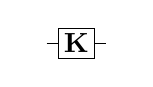
\begin{tikzpicture}[baseline={([yshift=-.5ex]current bounding box.center)}]
	\path (0,0) node (A) {}
	++ (0.5,0) node[kernel] (K) {$\kernel{K}$}
	++ (0.5,0) node (B) {};
	\draw (A) -- (K) -- (B);
\end{tikzpicture}\\
\kernel{P}&:= 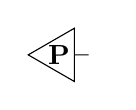
\begin{tikzpicture}[baseline={([yshift=-.5ex]current bounding box.center)}]
	\path (0,0) node[dist] (K) {$\kernel{P}$}
	++ (0.5,0) node (B) {};
	\draw (K) -- (B);
\end{tikzpicture}
\end{align}

Two Markov kernels $\kernel{L}:X\kto Y$ and $\kernel{M}:Y\kto Z$ have a product $\kernel{L}\kernel{M}:X\kto Z$ given by the matrix product $\kernel{L}\kernel{M}_x^z = \sum_y \kernel{L}_x^y\kernel{M}_y^z$. Graphically, we write represent by joining wires together:

\begin{align}
	\kernel{L}\kernel{M}:= 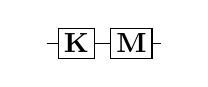
\begin{tikzpicture}[baseline={([yshift=-.5ex]current bounding box.center)}]
	\path (0,0) node (A) {}
	++ (0.5,0) node[kernel] (K) {$\kernel{K}$}
	++ (0.7,0) node[kernel] (M) {$\kernel{M}$}
	++ (0.5,0) node (B) {};
	\draw (A) -- (K) -- (M) -- (B);
\end{tikzpicture}
\end{align}

The Cartesian product $X\times Y:=\{(x,y)|x\in X, y\in Y\}$. Given kernels $\kernel{K}:W\kto Y$ and $\kernel{L}:X\kto Z$, the tensor product $\kernel{K}\otimes\kernel{L}:W\times X\kto Y\times Z$ is defined by $(\kernel{K}\otimes\kernel{L})_{(w,x)}^{(y,z)}:=K_{w}^y L_{x}^z$ and represents applying the kernels in parallel to their inputs.

The tensor product is represeted by drawing kernels in parallel:

\begin{align}
	\kernel{K}\otimes \kernel{L}&:=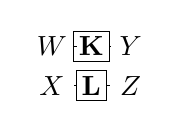
\begin{tikzpicture}[baseline={([yshift=-.5ex]current bounding box.center)}]
	\path (0,0) node (A) {$W$}
	++ (0.5,0) node[kernel] (K) {$\kernel{K}$}
	++ (0.5,0) node (B) {$Y$};
	\path (0,-0.5) node (C) {$X$}
	++ (0.5,0) node[kernel] (L) {$\kernel{L}$}
	++ (0.5,0) node (D) {$Z$};
	\draw (A) -- (K) -- (B);
	\draw (C) -- (L) -- (D);
\end{tikzpicture}
\end{align}

We read diagrams from left to right (this is somewhat different to \citet{fritz_synthetic_2020,cho_disintegration_2019,fong_causal_2013} but in line with \citet{selinger_survey_2010}). A diagram describes products and tensor products of Markov kernels, which are expressed according to the conventions described above. There are a collection of special Markov kernels for which we can replace the generic ``box'' of a Markov kernel with a diagrammatic elements that are visually suggestive of what these kernels accomplish.

A description of these kernels follows.

The identity map $\text{id}_X:X\kto X$ defined by $(\text{id}_X)_x^{x'}= \llbracket x = x' \rrbracket$, where the iverson bracket $\llbracket \cdot \rrbracket$ evaluates to $1$ if $\cdot$ is true and $0$ otherwise, is a bare line:

\begin{align}
	\mathrm{id}_X&:=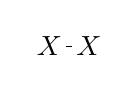
\begin{tikzpicture}[baseline={([yshift=-.5ex]current bounding box.center)}]
	\path (0,0) node (A) {$X$} ++ (0.5,0) node (B) {$X$};
	\draw (A) -- (B);
\end{tikzpicture}
\end{align}

We choose a particular 1-element set $\{*\}$ that acts as the identity in the sense that $\{*\}\times A=A\times \{*\} = A$ for any set $A$. The erase map $\text{del}_X:X\kto \{*\}$ defined by $(\text{del}_X)_x^* = 1$ is a Markov kernel that ``discards the input'' (we will later use it for marginalising joint distributions). It is drawn as a fuse:

\begin{align}
	\text{del}_X&:=\begin{tikzpicture}[baseline={([yshift=-.5ex]current bounding box.center)}]
	\path (0,0) ++ (1,0) node (B) {$X$};
	\draw[-{Rays[n=8]}] (A) -- (B);
\end{tikzpicture}
\end{align}

The copy map $\text{copy}_X:X\kto X\times X$ defined by $(\text{copy}_X)_x^{x',x''}=\llbracket x=x' \rrbracket \llbracket x=x'' \rrbracket$ is a Markov kernel that makes two identical copies of the input. It is drawn as a fork:

\begin{align}
	\text{copy}_X&:=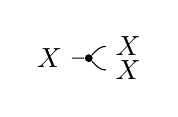
\begin{tikzpicture}[baseline={([yshift=-.5ex]current bounding box.center)}]
	\path (0,0) node (A) {$X$} 
	++ (0.5,0) node[copymap] (copy0) {}
	++ (0.5,0.15) node (B) {$X$}
	+ (0,-0.3) node (C) {$X$};
	\draw (A) -- (copy0) to [out=45,in=180] (B) (copy0) to [out=-45, in=180] (C);
\end{tikzpicture}
\end{align}

The swap map $\text{swap}_{X,Y}:X\times Y\kto Y\times X$ defined by $(\text{swap}_{X,Y})_{x,y}^{y',x'}=\llbracket x=x' \rrbracket\llbracket y=y' \rrbracket$ swaps two inputs, and is represented by crossing wires:

\begin{align}
	\text{swap}_X &:=  
\begin{tikzpicture}[baseline={([yshift=-.5ex]current bounding box.center)}]
		\path (0,0) node (A) {} 
		+ (0,-0.5) node (B) {}
		++ (1,0) node (C) {}
		+ (0,-0.5) node (D) {};
		\draw (A) to [out=0,in=180] (D) (B) to [out=0, in=180] (C);
	\end{tikzpicture}
\end{align}

Because we anticipate that the graphical notation will be unfamiliar to many, we will also include translations to more familiar notation.

\subsection{Truncated factorisation with Markov kernels}

The Markov kernels introduced in the previous section can be though of as ``conditional probability distributions without variables''. We can use these to represent an operation very similar to Equation \ref{eq:truncated_fac}. Note that $P^{\RV{Y|XZ}}$ must be represented by a Markov kernel $\kernel{K}:X\times Z\kto Y$ and $\prob{P}^{\RV{Z}}$ by a Markov kernel $\kernel{L}\in \Delta(Z)$. Then we can define a Markov kernel $\kernel{M}:X\kto X\times Z$ representing $x\mapsto \prob{P}^{\RV{YZ}}_{x}(y,z)$ by

\begin{align}
	\kernel{M}:= \tikzfig{truncated_factorisation}\label{eq:tfac_setted}
\end{align}

There is, however, a key difference between Equation \ref{eq:tfac_setted} and Equation \ref{eq:truncated_fac}: the Markov kernels in the latter equation describe the distribution of particular variables, while the former equation describes Markov kernels only.

To illustrate why we need variables, consider an arbitrary Markov kernel $\kernel{K}:\{*\}\kto \Delta(X\times X)$. We could draw this:
\begin{align}
	\kernel{K}:= \tikzfig{double_label}\label{eq:double_label}
\end{align}
We label both wires with the set $X$. However, say $X=\{0,1\}$. Then $\kernel{K}$ could be the kernel $\kernel{K}^{x_1,x_2} = \llbracket x_1 = 0\rrbracket \llbracket x_2 = 1\rrbracket$. In this case, both of its outputs must represent \emph{different} variables, despite taking values in the same set. On the other hand, if $\kernel{K}^{x_1,x_2} = 0.5 \llbracket x_1 = x_2 \rrbracket$ then both outputs coudl represent the same variable, because they are deterministically the same, or they could represent different variables that happen to be equal. We need some way to distinguish the two cases.


\subsection{Composition and probability with variables}

Our goal is to define a category of ``finite sets and Markov kernels with variables''. Introducing variables requires an assumption of consistency, which we don't know how to express in category theoretic terms. Our approach is to define a category of Markov kernels with variables that may or may not be consistent, which we will need to check for the resulting models. Because the consistency assumption is not expressed category theoretically, many proofs in this section only apply to our chosen setting of finite sets.

\begin{definition}[Variable]
Given a \emph{sample space} $\Omega$, a variable $f_\RV{X}$ is a function $\Omega\to A$ where $A$ is a vector space. We will also refer to the associated Markov kernel $\RV{X}:\Omega\kto A$
as a variable, where $\RV{X}_x^a=\llbracket a = f_{\RV{X}}(x) \rrbracket$.
\end{definition}

We define the \emph{product} of two variables as follows:
\begin{itemize}
	\item \textbf{Product:} Given variables $\RV{W}:\Omega\kto A$ and $\RV{V}:\Omega\kto B$, the product is defined as $(\RV{W}, \RV{V})=\text{copy}_{\Omega} (\RV{W}\otimes\RV{V})$
\end{itemize}

The \emph{unit} variable is the erase map $\RV{I}:=\text{del}_\Omega$, with $(\RV{I},\RV{X})=(\RV{X},\RV{I})=\RV{X}$ (up to isomorphism) for any $\RV{X}$.

We then need a notion of Markov kernels that ``maps between variables''. An \emph{indexed Markov kernel} is such a thing.

\begin{definition}[Indexed Markov kernel]
Given variables $\RV{X}:\Omega\to A$ and $\RV{Y}:\Omega\to B$, an indexed Markov kernel $\kernel{K}:\RV{X}\kto \RV{Y}$ is a triple $(\kernel{K}',\RV{X},\RV{Y})$ where $\kernel{K}':A\kto B$ is the \emph{underlying kernel}, $\RV{X}$ is the \emph{input index} and $\RV{Y}$ is the \emph{output index}.
\end{definition}

For example, if $\kernel{K}:(\RV{A}_1,\RV{A}_2)\to \Delta(\RV{B}_1,\RV{B}_2)$, for example, we can draw:

\begin{align}
	\kernel{K} := 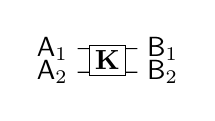
\begin{tikzpicture}[baseline={([yshift=-.5ex]current bounding box.center)}]
	\path (0,0) node (A1) {$\RV{A}_1$}
	+ (0,-0.3) node (A2) {$\RV{A}_2$}
	++ (0.7,-0.15) node[kernel] (K) {$\kernel{K}$}
	++ (0.7,0.15) node (B1) {$\RV{B}_1$}
	+ (0,-0.3) node (B2) {$\RV{B}_2$};
	\draw (A1) -- ($(K.west) + (0,0.15)$) (A2) -- ($(K.west) + (0,-0.15)$);
	\draw (B1) -- ($(K.east) + (0,0.15)$) (B2) -- ($(K.east) + (0,-0.15)$);
\end{tikzpicture}
\end{align}

or

\begin{align}
	\kernel{K} = 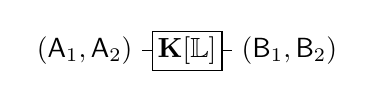
\begin{tikzpicture}[baseline={([yshift=-.5ex]current bounding box.center)}]
	\path (0,0) node (A1) {$(\RV{A}_1,\RV{A}_2)$}
	++ (1.3,0) node[kernel] (K) {$\kernel{K}[\model{L}]$}
	++ (1.3,0.) node (B1) {$(\RV{B}_1,\RV{B}_2)$};
	\draw (A1) -- (K) -- (B1);
\end{tikzpicture}
\end{align}

We define the product of indexed Markov kenrnels $\kernel{K}:\RV{X}\kto \RV{Y}$ and $\kernel{L}:\RV{Y}\kto \RV{Z}$ as the triple $\kernel{K}\kernel{L}:=(\kernel{K}'\kernel{L}',\RV{X},\RV{Z})$.

Similarly, the tensor product of $\kernel{K}:\RV{X}\kto\RV{Y}$ and $\kernel{L}:\RV{W}\kto\RV{Z}$ is the triple $\kernel{K}\otimes\kernel{L}:=(\kernel{K}'\otimes\kernel{L}',(\RV{X},\RV{W}),(\RV{Y},\RV{Z}))$.

We define $\text{Id}_{\RV{X}}$ to be the model $(\text{Id}_X,\RV{X},\RV{X})$, and similarly the indexed versions $\text{del}_{\RV{X}}$, $\text{copy}_{\RV{X}}$ and $\text{swap}_{\RV{X},\RV{Y}}$ are obtained by taking the unindexed versions of these maps and attaching the appropriate random variables as indices. Diagrams are the diagrams associated with the underlying kernel, with input and output wires annotated with input and output indices.

The category of indexed Markov kernels as morphisms and variables as objects is a Markov category (Appendix \ref{sec:app_mcat}), and so a valid derivation based on the string diagram language for Markov categories corresponds to a valid theorem in this category. However, most of the diagrams we can form are not viable candidates for models of our variables. For example, if $\RV{X}$ takes values in $\{0,1\}$ we can propose an indexed Markov kernel $\kernel{K}:\RV{X}\kto\RV{X}$ with $\kernel{K}_a^{\prime b}=0.5$ for all $a, b$. However, this is not a useful model of the variable $\RV{X}$ -- it expresses something like ``if we know the value of $\RV{X}$, then we belive that $\RV{X}$ could take any value with equal probability''.

We define a \emph{model} as ``an indexed Markov kernel that assigns probability 0 to things known to be contradictions''. A contradiction is a simultaneous assignment of values to the variables $\RV{X}$ and $\RV{Y}$ such that there is no value of $\omega$ under which they jointly take these values. Unless the value assignment to the domain variable is itself contradictory, we hold that any valid model must assign probability zero to such occurrences.

\begin{definition}[Probabilistic model]
An indexed Markov kernel $(\kernel{K}',\RV{X},\RV{Y})$ is a \emph{probabilistic model} (``model'' for short) if it is \emph{consistent}, which means it assigns probability 0 to contradictions:
\begin{align}
	f_{\RV{X}}^{-1}(a)\cap f_{\RV{Y}}^{-1}(b) = \emptyset \implies \left(\kernel{K}_{a}^{\prime b} = 0\right) \lor \left(f_{\RV{X}}^{-1}(a) = \emptyset\right)
\end{align}
A \emph{probability model} is a model where the underlying kernel $\kernel{K}'$ has the unit $\RV{I}$ as the domain. We use the font $\model{K}$ to distinguish models from arbitrary indexed Markov kernels.
\end{definition}

Consistency implies that for any $\model{K}:\RV{X}\kto\RV{Y}$, if $f_{\RV{Y}}=g\circ f_{\RV{X}}$ then $\model{K}_x^{g(x)}=1$. A particularly simple case of this is a model $\model{L}:\RV{X}\kto\RV{X}$, which must be such that $\model{L}_x^x=1$. \citet{hajek_what_2003} has pointed out that standard definitions of conditional probability allow the conditional probability to be arbitrary on a set of measure zero, even though ``the probability $\RV{X}=x$, given $\RV{X}=x$'' should obviously be 1.

We take the idea of marginal distributions as fundamental.

\begin{definition}[Marginal distribution]
Given a model $\model{K}:\RV{X}\kto(\RV{Y},\RV{Z})$, the marginal distribution of $\RV{Y}$, written $\model{K}^{\RV{Y}|\RV{X}}$, is obtained by marginalising over $\RV{Z}$:
\begin{align}
	\model{K}^{\RV{Y}|\RV{X}} &:= \tikzfig{marginal}\\
	&\iff\\
	(\model{K}^{\RV{Y}|\RV{X}})_x^y &= \sum_{z\in Z} \kernel{K}_x^{\prime yz}
\end{align}
\end{definition}

\begin{definition}[Disintegration]
Given a model $\model{K}:\RV{X}\kto(\RV{Y},\RV{Z})$, a disintegration $\model{L}:(\RV{X},\RV{Y})\kto \RV{Z}$ $\RV{Y}$, written $\model{K}^{\RV{Y}|\RV{X}}$, is obtained by marginalising over $\RV{Z}$
\end{definition}

We can always get a valid model by adding a copy map to a valid model, and conversely all valid models with repeated codomain variables must contain copy maps.

\begin{lemma}[Output copies of the same variable are identical]\label{lem:nocopy1}
For any $\kernel{K}:\RV{X}\kto (\RV{Y},\RV{Y},\RV{Z})$, $\kernel{K}$ is a model iff there exists some $\model{L}:\RV{X}\kto (\RV{Y},\RV{Z})$ such that
\begin{align}
		\kernel{K} &= \tikzfig{compose_with_copymap}\\
		&\iff \\
		\kernel{K}_{x}^{\prime y,y',z} &= \llbracket y=y' \rrbracket\kernel{L}_{x}^{\prime y,z}\\
\end{align}
\end{lemma}


\begin{proof}
$\implies$
For any $\omega,x,y,y',z$:
\begin{align}
	(\RV{X},\RV{Y},\RV{Y},\RV{Z})_\omega^{x,y,y',z} &= \llbracket f_{\RV{Y}}(\omega)=y \rrbracket \llbracket f_{\RV{Y}}(\omega)=y' \rrbracket (\RV{X},\RV{Z})_\omega^{x,z} \\
	&= \llbracket y=y' \rrbracket \llbracket f_{\RV{Y}}(\omega)=y \rrbracket(\RV{X},\RV{Z})_\omega^{x,z}
\end{align}
Therefore, by consistency, for any $x,y,y',z$, $y\neq y'\implies \kernel{K}_{x}^{\prime yy'z}=0$. Define $\kernel{L}$ by $\kernel{L}_x^{\prime y, z} := \kernel{K}_x^{\prime y y z}$. The fact that $\model{L}$ is a model follows from the assumption that $\model{K}$ is. Then
\begin{align}
	\kernel{K}_{x}^{\prime y,y',z} &= \llbracket y=y' \rrbracket\kernel{L}_{x}^{\prime y,z}
\end{align}
$\Leftarrow$
If $\model{L}$ is a model, then for any $x,x',y,z$, 
\begin{align}
\llbracket y=y'\rrbracket \model{L}_{x}^{\prime y,z}>0&\implies y=y'\land \model{L}_{x}^{\prime y,z}>0\\
													  &\implies \left(f_{\RV{X}}^{-1}(x)=\emptyset \right)\lor \left(f_{\RV{X}}^{-1}(x)\cap f_{\RV{Y}}^{-1}(y) \cap f_{\RV{Y}}^{-1}(y)\cap f_{\RV{Z}}^{-1}(z)\neq\emptyset \right)\\
\end{align}
\end{proof}

We can always get a valid model by copying the input to the output of a valid model, and conversely all valid models where there is a variable shared between the input and the output must copy that input to the output.

\begin{lemma}[Copies shared between input and output are identical]\label{lem:nocopy2}
For any $\kernel{K}:(\RV{X},\RV{Y})\kto (\RV{X},\RV{Z})$, $\kernel{K}$ is a model iff there exists some $\model{L}:(\RV{X},\RV{Y})\kto \RV{Z}$ such that
\begin{align}
	 \kernel{K} &= \tikzfig{precompose_with_copymap}\\
	 &\iff\\
	 \kernel{K}_{x,y}^{\prime x',z} &= \llbracket x=x'\rrbracket \kernel{L}_{\prime x,y}^{z}
\end{align}
\end{lemma}

\begin{proof}
$\implies$
For any $\omega,x,y,y',z$:
\begin{align}
	(\RV{X},\RV{Y},\RV{Y},\RV{Z})_\omega^{x,y,y',z} &= \llbracket f_{\RV{Y}}(\omega)=y \rrbracket \llbracket f_{\RV{Y}}(\omega)=y' \rrbracket (\RV{X},\RV{Z})_\omega^{x,z} \\
	&= \llbracket y=y' \rrbracket \llbracket f_{\RV{Y}}(\omega)=y \rrbracket(\RV{X},\RV{Z})_\omega^{x,z}
\end{align}
Therefore, by consistency, for any $x,y,y',z$, $x\neq x'\implies \model{K}_{x,y}^{\prime x'z}=0$. Define $\kernel{L}$ by $\kernel{L}_{x,y}^{\prime x', z} := \model{K}_{x,y}^{\prime x, y}$. The fact that $\kernel{L}$ is a model follows from the assumption that $\model{K}$ is a model. Then
\begin{align}
	\kernel{K}_{x, y}^{\prime x', z} &= \llbracket x=x' \rrbracket\kernel{L}_{x,y}^{\prime z}
\end{align}
$\Leftarrow$
If $\model{L}$ is a model, then for any $x,x',y,z$, 
\begin{align}
\llbracket x=x'\rrbracket \model{L}_{ x,y}^{\prime z}>0&\implies x=x'\land \model{L}_{ x,y}^{\prime z}>0\\
													  &\implies \left( f_{\RV{X}}^{-1}(x)\cap f_{\RV{Y}}^{-1}(y)=\emptyset \right)\lor \left(f_{\RV{X}}^{-1}(x)\cap f_{\RV{X}}^{-1}(x)\cap f_{\RV{Y}}^{-1}(y)\cap f_{\RV{Z}}^{-1}(z)\neq\emptyset \right)\\
\end{align}
\end{proof}

Consistency along with the notion of marginal distributions implies that, given some $\RV{X}$ and some $\model{K}:\RV{Y}\kto\text{Id}_\Omega$, the pushforward $\model{K}\model{X}$ is the unique model $\RV{Y}\kto \RV{X}$ that can be paired (Definition \ref{def:pairing}) with $\model{K}$. This is shown in Lemma \ref{lem:pushforward}.

\begin{lemma}[Uniqueness of models with the sample space as a domain]\label{lem:uniq_model}
For any $\RV{X}:\Omega\to A$, there is a unique model $\model{X}:\text{Id}_\Omega\kto \RV{X}$ given by $\model{X}:=(\RV{X},\text{Id}_\Omega,\RV{X})$.
\end{lemma}

\begin{proof}
$\RV{X}$ is a Markov kernel mapping from $\Omega\to A$, so it is a valid underlying kernel for $\model{X}$, and $\model{X}$ has input and output indices matching its signature. We need to show it satisfies consistency.

For any $\omega\in \Omega$, $a\in A$
\begin{align}
	\max_{\omega\in \Omega}(\text{Id}_\Omega,\RV{X})_{\omega}^{\omega',a} &= \max_{\omega\in \Omega} \llbracket \omega = \omega' \rrbracket \llbracket \omega = f_{\RV{X}}(a) \rrbracket\\
	&= \llbracket \omega = f_{\RV{X}}(a) \rrbracket\\
	&= \kernel{X}_\omega^a
\end{align}
Thus $\model{X}$ satisfies consistency.

Suppose there were some $\model{K}:\text{Id}_\Omega\kto \RV{X}$ not equal to $\RV{X}$. Then there must be some $\omega\in \Omega$, $b\in A$ such that $\model{K}_\omega^b\neq 0$ and $f_{\RV{X}}(\omega)\neq b$. Then
\begin{align}
	\max_{\omega\in \Omega}(\text{Id}_\Omega,\RV{X})_{\omega}^{\omega',a} &= \max_{\omega\in \Omega} \llbracket \omega = \omega' \rrbracket \llbracket \omega = f_{\RV{X}}(b) \rrbracket\\
	&= \llbracket \omega = f_{\RV{X}}(b) \rrbracket\\
	&= 0\\
	&< \model{K}_\omega^b
\end{align}
Thus $\model{K}$ doesn't satisfy consistency.
\end{proof}

% \begin{corollary}[Uniqueness of joint models]\label{cor:uniq_joint}
% For any $\RV{X}:\Omega\to A$, there is a unique model $\model{X}:\text{Id}_\Omega\kto (\RV{X},\text{Id}_{\Omega})$.
% \end{corollary}

% \begin{proof}
% Apply Lemma \ref{lem:nocopy2} to the model $\model{X}$ from Lemma \ref{lem:uniq_model}.
% \end{proof}

\begin{definition}[Pairing]\label{def:pairing}
Two models $\model{K}:\RV{X}\kto \RV{Y}$ and $\model{L}:\RV{X}\kto \RV{Z}$ can be \emph{paired} if there is some $\model{M}:\RV{X}\kto (\RV{Y},\RV{Z})$ such that $\model{K}=\model{M}^{\RV{Y}|\RV{X}}$ and $\model{L}=\model{M}^{\RV{Z}|\RV{X}}$.
\end{definition}

\begin{lemma}[Pushforward model]\label{lem:pushforward}
Given any model $\model{K}:\RV{Y}\kto \text{Id}_\Omega$ and any $\RV{X}$, there is a unique $\model{L}:\RV{Y}\kto \RV{X}$ that can be paired with $\model{K}$, and it is given by $(\kernel{L}^a_b = \sum_{\omega\in f_{\RV{X}}^{-1}(a)} \kernel{K}_b^{\omega}$.
\end{lemma}

\begin{proof}
Suppose that there is some $\model{L}$ that can be paired with $\model{K}$ via some $\model{M}:\RV{Y}\kto(\text{Id}_\Omega,\RV{X})$. Then, by the existence of disintegrations, there must be some $\model{N}:\text{Id}_{\Omega}\kto \RV{X}$ such that
\begin{align}
	\model{M}&=\tikzfig{disintegration_omega}
\end{align}
By Corollary \ref{cor:uniq_joint}, there is only one model $\model{N}:\text{Id}_{\Omega}\kto \RV{X}$ is unique and equal to $\model{X}:=(\RV{X},\text{Id}_\Omega,\RV{X})$.

It remains to be shown that $\model{M}$ is also a model. We already know that $\model{K}$ is consistent with respect to $(\RV{Y},\text{Id}_\Omega)$ and $\model{L}$ is consistent with respect to $(\text{Id}_\Omega,\RV{X})$. $\model{M}$ must be consistent with respect to $(\RV{Y},\text{Id}_\Omega,\RV{X})$. Consider any $x\in X$, $\omega\in \Omega$, $y\in Y$ such that $f_{\RV{X}}^{-1}(x)\cap \{\omega\}\neq \emptyset$ and $f_{\RV{Y}}^{-1}(y)\cap\{\omega\}\neq \emptyset$. Trouble might arise if $f_{\RV{X}}^{-1}(x)\cap \{\omega\} \cap f_{\RV{Y}}^{-1}(y)=\emptyset$, but this is obviously impossible as $\omega\in f_{\RV{X}}^{-1}(x)$ and $\omega\in f_{\RV{Y}}^{-1}(y)$.

Finally, for any $a\in A$, $b\in B$
\begin{align}
	(\model{K}\model{X})^a_b &= \sum_{\omega\in \Omega} \model{P}_b^\omega\RV{X}_\omega^a\\
						 &= \sum_{\omega\in \Omega} \model{P}_b^\omega \llbracket a = f_{\RV{X}}(\omega) \rrbracket\\
						 &= \sum_{\omega\in f^{-1}(a)} \model{P}_b^{\omega}
\end{align}
\end{proof}

\begin{corollary}[Pushforward probability model]\label{corr:pushforward}
Given any probability model $\model{P}:\RV{I}\kto \text{Id}_\Omega$, there is a unique model $\model{P}^{\RV{X}}:\RV{I}\kto \RV{X}$ such that $\model{P}^{\RV{X}}=\model{P}\model{Q}$ for some $\model{Q}:\text{Id}_\Omega\to \RV{X}$, and it is given by $(\model{P}^{\RV{X}})^a_b = \sum_{\omega\in f^{-1}(a)} \model{P}_b^{\omega}$.
\end{corollary}

\begin{proof}
Apply Lemma \ref{lem:pushforward} to a model $\model{P}:\RV{I}\kto\text{Id}_{\Omega}$.
\end{proof}

The following lemmas can help us check whether an indexed Markov kernel is a valid model.



We take the following term from \citet{constantinou_extended_2017}. Our definition is equivalent to unconditional variation independence in that paper.

\begin{definition}[Variation independence]
Two variables $\RV{X}:\Omega\kto X$ and $\RV{Y}:\Omega\kto Y$ are variation independent, written $\RV{X}\perp_v \RV{Y}$, if for all $y\in f_\RV{Y}(\Omega)R(f_{\RV{Y}})$
\begin{align}
 f_\RV{Y}(\Omega) \times f_{\RV{X}}(\Omega) = \{(f_{\RV{Y}}(\omega),f_{\RV{X}}(\omega))|\omega\in \Omega\}
\end{align}
\end{definition}

If a collection of variables is variation independent and surjective, then an arbitrary indexed Markov kernel labelled with these variables is a model.

\begin{lemma}[Consistency via variation conditional independence]\label{lem:var_indep}
Given an indexed Markov kernel $\kernel{K}:\RV{X} \kto \RV{Y}$ with $\RV{X}:\Omega\kto X$ and $\RV{Y}:\Omega\kto Y$, if $f_\RV{Y}$ is surjective and $\RV{Y}\perp_v \RV{X}$ then $\kernel{K}$ is a model.
\end{lemma}

\begin{proof}
By variation independence and surjectivity of $f_{\RV{Y}}$, for any $x\in X$, $y\in Y$, $f_{\RV{X}}^{-1}(x)\cap f_{\RV{Y}}^{-1}(y) = \emptyset \implies f_{\RV{X}}^{-1}(x) = \emptyset$. Thus the criterion of consistency places no restrictions on $\kernel{K}$.
\end{proof}

\todo[inline]{I think Lemmas \ref{lem:nocopy1} and \ref{lem:nocopy2} might be sufficient to offer diagrammatic checks of consistency if all variables that are not identical are variation independent. This is probably an interesting result, but I'm not sure if it's a higher priority than filling out the rest of the content.}

Alternatively, if we have a strictly positive indexed Markov kernel that is known to be a model, we can conclude that arbitrary indexed Markov kernels with appropriate labels are also models.

\begin{lemma}[Consistency via positive models]\label{lem:avoid_contradic}
Given a model $\model{K}:\RV{X}\kto (\RV{Y},\RV{Z})$, if an indexed Markov kernel $\kernel{L}:(\RV{X},\RV{Y})\kto \RV{Z}$ has the property $\kernel{K}_x^{\prime yz}=0\implies \kernel{L}_{xy}^{\prime z}=0$ then $\kernel{L}$ is also a model.
\end{lemma}

\begin{proof}
Because $\model{K}$ is a model,
\begin{align}
	\kernel{L}_{xy}^{\prime z}>0 &\implies \kernel{K}_x^{\prime yz} >0 \\
	&\implies \left( f_\RV{X}^{-1}(x)\cap f_\RV{Y}^{-1}(y)\cap f_\RV{Z}^{-1}(z) \neq \emptyset \right) \lor \left(f_\RV{X}^{-1}(x) = \emptyset \right)\\
	&\implies \left( f_\RV{X}^{-1}(x)\cap f_\RV{Y}^{-1}(y)\cap f_\RV{Z}^{-1}(z) \neq \emptyset \right) \lor \left(f_\RV{X}^{-1}(x)\cap f_{\RV{Y}}^{-1}(y) = \emptyset \right)
\end{align}
\end{proof}

\subsection{Truncated factorisation with variables}

At this point, we can represent Equation \ref{eq:truncated_fac} using models. Suppose $P^{\RV{Y|XZ}}$ is an model $\model{K}:(\RV{X}, \RV{Z})\kto \RV{Y}$ and $\prob{P}^{\RV{Z}}$ an model $\model{L}:\{*\}\kto \RV{Z}$. Then we can define an indexed Markov kernel $\kernel{M}:\RV{X}\kto \RV{X}, \RV{Z}$ representing $x\mapsto \prob{P}^{\RV{YZ}}_{x}(y,z)$ by

\begin{align}
	\kernel{M}&:= \tikzfig{truncated_factorisation_labeled}\label{eq:tfac_labeled}
\end{align}

Equation \ref{eq:tfac_labeled} is almost identical to Equation \ref{eq:tfac_setted}, except it now specifies which variables each measure applies to, not just which sets they take values in. Like the original Equation \ref{eq:truncated_fac}, there is no guarantee that $\kernel{M}$ is actually a model. If $f_\RV{X}=g\circ f_\RV{Z}$ for some $g:Z\to X$ and $X$ has more than 1 element, then the rule of consistency will rule out the existence of any such model.

If we want to use $\kernel{M}$, we want it at minimum to satisfy the consistency condition. One approach we could use is to check the result using Lemmas \ref{lem:nocopy1} to \ref{lem:avoid_contradic}, although note that \ref{lem:var_indep} and \ref{lem:avoid_contradic} are sufficient conditions, not necessary ones.

\subsection{Sample space models and submodels}

Instead of trying to assemble probability models as in Equation \ref{eq:tfac_labeled}, we might try to build probability models in a manner closer to the standard setup -- that is, we start with a sample space model (or a collection of sample space models) and work with marginal and conditional probabilities derived from these, without using any non-standard model assemblies.

A sample space model is any model $\kernel{K}:\RV{X}\kto \text{Id}_\Omega$. We expect that the collection of models under consideration will usually be defined on some small collection of random variables, but every such model is the pushforward of some sample space model. Using sample space models allows us to stay close to the usual convention of probability modelling that starts with a sample space probability model.

\begin{lemma}[Existence of sample space model]\label{lem:ss_exist}
Given any model $\model{K}:\RV{X}\kto \RV{Y}$, there is a sample space model $\model{L}:\RV{X}\kto\text{Id}_\Omega$ such that, defining $\model{Y}:=(\RV{Y},\text{Id}_\Omega,\RV{Y})$, $\model{L}\model{Y}=\model{K}$.
\end{lemma}

\begin{proof}
If $\RV{X}:\Omega\kto A$ and $\RV{Y}:\Omega\kto B$, take any $a\in A$ and $b\in B$. Then set

\begin{align}
	\kernel{L}_a^{\prime \omega} = \begin{cases}
					0 & \text{ if } f_{\RV{Y}}^{-1}(b)\cap f_{\RV{X}}^{-1}(a)=\emptyset\\
					\kernel{K}_a^{\prime b} \llbracket \omega = \omega_b \rrbracket & \text{for some }\omega_b\in f_{\RV{Y}}^{-1}(b) \text{ if }f_{\RV{X}}^{-1}(a)=\emptyset\\
					\kernel{K}_a^{\prime b} \llbracket \omega = \omega_{ab} \rrbracket & \text{for some }\omega_{ab}\in f_{\RV{Y}}^{-1}(b)\cap f_{\RV{X}}^{-1}(a)\text{ otherwise}\\
					\end{cases}
\end{align}

Note that for all $a\in A$, $\sum_{\omega\in \Omega}\kernel{L}^{\prime\omega}_a = \sum_{b\in B} \kernel{K}_a^{\prime b} = 1$.

By construction, $(\kernel{L}',\text{Id}_\Omega,\RV{X})$ is free of contradiction. In addition
\begin{align}
	(\kernel{L}'\RV{Y})_a^b &= \sum_{\omega\in \Omega} \kernel{L}^{\prime \omega}_a \RV{Y}_\omega^b\\
							&= \sum_{\omega\in f_{\RV{Y}}^{-1}(b)} \kernel{L}_a^{\prime \omega}\\
							&= \begin{cases}
							 0 & f_{\RV{Y}}^{-1}(b)\cap f_{\RV{X}}^{-1}(a)=\emptyset\\
							 \kernel{K}_a^{\prime b} & \text{ otherwise }
							\end{cases}\\
		\implies (\kernel{L}'\RV{Y}) &= \kernel{K}'
\end{align}
\end{proof}

\begin{definition}[Pushforward model]
For any variables $\RV{X}:\Omega\kto A$, $\RV{Y}:\Omega\kto B$ and any sample space model $\model{K}:\RV{X}\kto \mathrm{Id}_\Omega$, the pushforward $\model{K}^{\RV{Y}|\RV{X}}:= \model{K}\model{X}$ where $\model{X}:=(\RV{X},\mathrm{Id}_\Omega,\RV{X})$.
\end{definition}

The fact that the pushforward is a model is proved in Lemma \ref{lem:pushforward}. We employ the slightly more familiar notation $\model{K}^{\RV{Y}|\RV{X}}(y|x)\equiv (\kernel{K}^{\prime \RV{Y}|\RV{X}})^y_x$.

\begin{definition}[Submodel]\label{def:submodel}
Given $\model{K}:\RV{X}\kto \mathrm{Id}_\Omega$ and $\model{L}:\RV{W,X}\kto \RV{Z}$, $\model{L}$ is a submodel of $\model{K}$ if
\begin{align}
	 \model{K}^{\RV{Z,W}|\RV{Y}} &= \tikzfig{conditional_submodel}\label{eq:submodel}\\
	 (\model{K}^{\RV{Z,W}|\RV{Y}})_x^{w,z} &= (\model{K}^{\RV{W}|\RV{Y}})_x^w\model{L}_{w,x}^z		  
\end{align}
We write $\model{L}\in \model{K}^{\{\RV{Z}|\RV{W},\RV{X}\}}$.
\end{definition}

\begin{lemma}[Submodel existence]\label{lem:subm_exist}
For any model $\model{K}:\RV{X}\kto \mathrm{Id}_\Omega$ (where $\Omega$ is a finite set), $\RV{W}$ and $\RV{Y}$, there exists a submodel $\model{L}:(\RV{W},\RV{X})\kto \RV{Y}$.
\end{lemma}

\begin{proof}
Consider any indexed Markov kernel $\kernel{L}:(\RV{W},\RV{X})\kto \RV{Y}$ with the property
\begin{align}
	\kernel{L}_{wx}^{\prime y} = \frac{\model{K}^{\RV{W,Y}|\RV{X}}(w,y|x)}{\model{K}^{\RV{W}|\RV{X}}(w|x)}\qquad\forall {x,w}:\text{ the denominator is positive}
\end{align}
In general there are many indexed Markov kernels that satisfy this. We need to check that $\kernel{L}'$ can be chosen so that it avoids contradictions. For all $x,y$ such that $\kernel{K}^{\RV{Y}|\RV{X}}(y|x)$ is positive, we have $\model{K}^{\RV{W,Y}|\RV{X}}(w,y|x)>0\implies \kernel{L}_{wx}^{\prime y} > 0$. Furthermore, where $\model{K}^{\RV{W}|\RV{X}}(w|x)=0$, we either have $f_{\RV{W}}^{-1}(w)\cap f_{\RV{X}}^{-1}(x)=\emptyset$ or we can choose some $\omega_{wx}\in f_{\RV{W}}^{-1}(w)\cap f_{\RV{X}}^{-1}(x)$ and let $\kernel{L}_{wx}^{\prime f_{\RV{Y}}(\omega_{wx})} = 1$. Thus $\kernel{L}'$ can be chosen such that $\kernel{L}$ is a model (but this is not automatic).

Then
\begin{align}
	\model{K}^{\RV{W}|\RV{X}}(w|x) \kernel{L}_{xw}^{\prime y} &= \model{K}^{\RV{W}|\RV{X}}(w|x) \frac{\model{K}^{\RV{W,Y}|\RV{X}}(w,y|x)}{\model{K}^{\RV{W}|\RV{X}}(w|x)} &\text{ if }\model{K}^{\RV{W}|\RV{X}}(w|x)>0\\
												   &= \model{K}^{\RV{W,Y}|\RV{X}}(w,y|x) &\text{ if }\model{K}^{\RV{W}|\RV{X}}(w|x)>0\\
												   &= 0 &\text{otherwise}\\
												   &= \model{K}^{\RV{W,Y}|\RV{X}}(w,y|x) &\text{otherwise}
\end{align}
\end{proof}

\subsection{Conditional independence}\label{ssec:cond_indep}

We define conditional independence in the following manner:

For a \emph{probability model} $\model{P}:\RV{I}\kto \text{Id}_{\Omega}$ and variables $(\RV{A},\RV{B},\RV{C})$, we say $\RV{A}$ is independent of $\RV{B}$ given $\RV{C}$, written $\RV{A}\CI_{\model{P}}\RV{B}|\RV{C}$, if

\begin{align}
	\kernel{P}^{\RV{ABC}} &= \tikzfig{cond_indep1}
\end{align}

For an arbitrary model $\kernel{N}:\RV{X}\kto \text{Id}_{\Omega}$ where $\RV{X}:\Omega\kto X$, and some $(\RV{A},\RV{B},\RV{C})$, we say $\RV{A}$ is independent of $\RV{B}$ given $\RV{C}$, written $\RV{A}\CI_{\kernel{N}}\RV{B}|\RV{C}$, if there is some $\model{O}:\RV{I}\kto \RV{X}$ such that $O^x>0$ for all $x\in f_{\RV{X}}^{-1}(X)$ and $\RV{A}\CI_{\model{O}\model{N}} \RV{B}|\RV{C}$.

This definition is inappliccable in the case where sets may be uncountably infinite, as no such $\kernel{O}$ can exist in this case. There may well be definitions of conditional independence that generalise better, and we refer to the discussions in \citet{fritz_synthetic_2020} and \citet{constantinou_extended_2017} for some discussion of alternative definitions. One advantage of this definition is that it matches the version given by \citet{cho_disintegration_2019} which they showed coincides with the standard notion of conditional independence and so we don't have to show this in our particular case.

A particular case of interest is when a kernel $\kernel{K}:(\RV{X},\RV{W})\to \Delta(\RV{Y})$ can, for some $\kernel{L}:\RV{W}\to \Delta(\RV{Y})$, be written:

\begin{align}
	\kernel{K} = \tikzfig{ci_example}
\end{align}

Then $\RV{Y}\CI_{\kernel{K}}\RV{W}|\RV{X}$.
%!TEX root = main.tex

\section{See-do models}\label{sec:seedo_models}

Modular probability is useful when we want to combine different Markov kernels in such a way that ``variables'' refer to something consistent even though they don't necessarily have a unique distribution. The first example we will present is using modular probability to model decision problems.

Suppose we will be given an observation $x\in X$ and in response to this we can select any decision or stochastic mixture of decisions from a set $D$; that is we can choose a ``strategy'' as any Markov kernel $\kernel{S}_\alpha:X\to \Delta(D)$. We are intersted in forecasting some consequences that take values in some set $Y$, and comparing the forecasts for different strategy choices so as to choose a best strategy.

How can we model this? One way to proceed is as follows: Define a model context $\mathscr{M}$ to which we add the conditional probabilities mentioned hereafter. For each strategy $\model{S}_\alpha[\RV{D}|\RV{X}]$, our forecast will be represented by some joint probability in $\model{P}_{\alpha}[\RV{X}\RV{D}\RV{Y}|\RV{H}]$ where $\RV{H}$ is associated with a set of hypotheses $H$ representing different choices that we think might be reasonable to make that may lead to different forecasts. Because observations come before we execute our strategy, we assume that $\model{P}_{\alpha}[\RV{X}|\RV{H}]=P_{\beta}[\RV{X}|\RV{H}]$ for all $\alpha,\beta$. Our chosen strategy is the probability of $\RV{D}$ given $\RV{X}$: $\model{P}_{\alpha}[\RV{D}|\RV{X}]\overset{krn}{=}\model{S}_\alpha[\RV{D}|\RV{X}]$. Finally, our forecast of $\RV{Y}$ is the same for all strategies holding the observations, the decision and the hypothesis fixed: $\model{P}_{\alpha}[\RV{Y}|\RV{HD}]=P_{\beta}[\RV{Y}|\RV{HD}]$ for all $\alpha,\beta$.

Under these assumptions, there exists $\model{T}[\RV{X}\RV{Y}|\RV{HD}]\in \mathscr{M}$ with $\RV{X}\CI_{\model{T}}\RV{D}|\RV{H}$ such that for all $\alpha$, 

\begin{align}
    \model{P}_{\alpha}[\RV{X}\RV{D}\RV{Y}|\RV{H}]\overset{krn}{=}\model{T}[\RV{X}|\RV{H}]\rightrightarrows \model{S}_\alpha [\RV{D}|\RV{X}] \rightrightarrows \model{T}[\RV{Y}|\RV{XHD}] \label{eq:see_do_query}
\end{align}

The proof is given in Appendix \ref{sec:see-do-rep}. Note that $\model{T}[\RV{X}|\RV{H}]$ exists by virtue of the fact $\RV{X}\CI_{\model{T}}\RV{D}|\RV{H}$. While this independence is what enables Equation \ref{eq:see_do_query}, in general $\RV{X}\not\CI_{\model{P}_\alpha} \RV{D}|\RV{H}$, so $\model{T}$ cannot be a disintegration of $\model{P}_\alpha$. Modular probability allows us to specify $\model{T}$, which we call a \emph{see-do model}, as a partial forecast to be completed with a strategy $\model{S}_\alpha$ while also being able to use consistent names for variables that represent the same things (observations, decisions, consequences, hypotheses) whether their distributions are given by $\model{P}_\alpha$, $\model{T}$, which are mutually incompatible conditional probabilities.

\subsection{See-do models and classical statistics}

A \emph{statistical model} (or \emph{statistical experiment}) is a collection of probability distributions indexed by some set $\Theta$. We can observe that $\{\model{T}[\RV{X}|\RV{H}]_h\}_{h\in H}$ is a collection of probability distributions indexed by $H$.

In statistical decision theory, as introduced by \citet{wald_statistical_1950}, we are given a statistical experiment $\{\prob{P}_\theta\in \Delta(X)\}_\Theta$, a decision set $D$ and a loss $l:\Theta\times D\to \mathbb{R}$. A strategy $\model{S}_\alpha:X\to \Delta(D)$ is evaluated according to the risk functional $R(\theta,\model{S}_\alpha)=\sum_{x\in X}\sum_{d\in D} \prob{P}_\theta^x (S_\alpha)_x^d l(h,d)$.

Suppose we have a see-do model $\model{T}[\RV{X}\RV{Y}|\RV{HD}]$ with $\RV{Y}\CI_{\kernel{T}} \RV{X}|\RV{HD}$, and suppose that the random variable $\RV{Y}$ is a ``reverse utility'' function taking values in $\mathbb{R}$ for which low values are considered desirable. Then, defining a loss $l:H\times D\to \mathbb{R}$ by $l(h,d) = \sum_{y\in \mathbb{R}} y\model{T}[\RV{Y}|\RV{H}\RV{D}]_{h,d}^y$, we have 

\begin{align}
    \mathbb{E}_{\model{P}_{\alpha}[\RV{X}\RV{D}\RV{Y}|\RV{H}]}[\RV{Y}] &= \sum_{x\in X} \sum_{d\in D} \sum_{y\in Y} y \left(\model{T}[\RV{X}|\RV{H}]\rightrightarrows \model{S}_\alpha [\RV{D}|\RV{X}] \rightrightarrows \model{T}[\RV{Y}|\RV{XHD}]\right)_h^{xdy}\\
     &= \sum_{x\in X} \sum_{d\in D} \sum_{y\in Y} \model{T}[\RV{X}|\RV{H}]^x_h \model{S}_\alpha [\RV{D}|\RV{X}]_x^d \model{T}[\RV{Y}|\RV{H}\RV{D}]_{h,d}^y\\
    &= \sum_{x\in X}\sum_{d\in D} \model{T}[\RV{X}|\RV{H}]_h^x (S_\alpha)_x^d l(h,d)\\
    &= R(h,\model{S}_\alpha)
\end{align}

That is, if we are given a see-do model where we interpret $\model{T}[\RV{X}|\RV{H}]$ as a statistical experiment and $\RV{Y}$ as a reversed utility, the expectation of the utility under the strategy forecast given in equation \ref{eq:see_do_query} is the risk of that strategy under hypothesis $h$.

\subsection{Combs}

The see-do model $\model{T}[\RV{X}\RV{Y}|\RV{HD}]$ is known as a \emph{comb}. This structure was introduced by \citet{chiribella_quantum_2008} in the context of quantum circuit architecture, and \citet{jacobs_causal_2019} adapted the concept to causal modelling.

A comb is a Markov kernel with a ``hole'' in it. We combine the see-do model with a strategy by putting the strategy ``in the middle'' of the see-do model (Equation \ref{eq:see_do_query}), rather than attaching it to one end. While it is not a well-formed diagram in the language described in this paper, we can visualise combs as Markov kernels with holes:

\begin{align}
\model{T}[\RV{XY}|\RV{HD}] &= 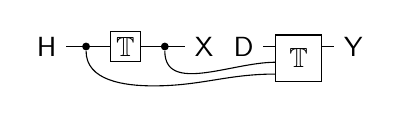
\begin{tikzpicture}
    \path (0,0) node (H) {$\RV{H}$}
     ++ (0.5,0) node[copymap] (copy0) {}
     ++ (0.5,0) node[kernel] (XH) {$\model{T}$}
     ++ (0.5,0) node[copymap] (copy1) {}
     ++ (0.5,0) node (X) {$\RV{X}$}
     ++ (0.5,0.) node (D) {$\RV{D}$}
     ++ (0.7,-0.15) node[kernel,inner sep=5pt] (YDXH) {$\model{T}$}
     ++ (0.7,0.15) node (Y) {$\RV{Y}$};
     \draw (H) -- (XH) -- (X) (D) to [out=0,in=180] ($(YDXH.west) + (0,0.15)$) ($(YDXH.east) + (0,0.15)$) -- (Y);
     \draw (copy0) to [out=-90,in=180] ($(copy0.east) + (0.8,-0.5)$) to [out=0,in=180] ($(YDXH.west) + (0,-0.2)$) (copy1) to [out=-90,in=180] ($(YDXH.west) + (0,-0.05)$);
\end{tikzpicture}\\
&= 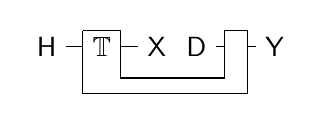
\begin{tikzpicture}
    \path (0,0) node (H) {$\RV{H}$}
     ++ (0.7,0) node (XH) {$\model{T}$}
     ++ (0.7,0) node (X) {$\RV{X}$}
     ++ (0.5,0) node (D) {$\RV{D}$}
     ++ (0.5,0) node[inner sep=4pt] (YDXH) {}
     ++ (0.5,0) node (Y) {$\RV{Y}$};
     \draw (H) -- (XH) -- (X) (D) -- (YDXH) -- (Y);
     \draw ($(XH.west) + (0,0.2)$) -- ($(XH.west) + (0,-0.6)$) -- ($(YDXH.east) + (0,-0.6)$)
     -- ($(YDXH.east) + (0,0.2)$) -- ($(YDXH.west) + (0,0.2)$) -- ($(YDXH.west) + (0,-0.4)$)
     -- ($(XH.east) + (0,-0.4)$) -- ($(XH.east) + (0,0.2)$) -- ($(XH.west) + (0,0.2)$);
\end{tikzpicture}\label{eq:kernel_with_hole}
\end{align}

We can take any strategy $\model{S}_\alpha[\RV{D}|\RV{X}]$ and drop it into the ``hole'' in \ref{eq:kernel_with_hole} (as described in Equation \ref{eq:see_do_query}) to get a forecast of the outcome of that strategy. 
%!TEX root = main.tex

\section{Repeatable experiments}

While there are types of measurement processes we could consider, statistical inference usually proceeds from repeatable measurement processes. A common precise notion of repeatability is the assumption of \emph{exchangeability}. The term ``exchangeability'', like the term random variable, is used to refer to assumptions about \emph{measurement processes} as well as properties of \emph{probability models}. If I say a measurement process $\proc{S}$ taking values in $S^n$ is exchangeable, I might mean:
\begin{itemize}
    \item I believe that there is some probabilistic model $(\prob{P},\Omega,\sigalg{F})$ and random variable $\RV{S}$ appropriate for modelling $\proc{S}$ and
    \begin{enumerate}
        \item The same model is appropriate for any measurement process that first peforms $\proc{S}$ and subsequently shuffles the results according to any permutation $\text{swap}_a:S^n\to S^n$ or
        \item The same model is appropriate for any measurement process related to $\proc{S}$ by interchanging experimental units or subjects in the real world
    \end{enumerate} 
\end{itemize}

On the other hand, if I say a probability model $(\prob{P},S^{|A|},\sigalg{S}^{|A|})$ is exchangeable, I mean

\begin{itemize}
    \item For any finite permutation $\text{swap}_A:S^{|A|}\kto S^{|A|}$, $\prob{P}^{\RV{S}}\text{swap}_{a} = \prob{P}^{\RV{S}}$
\end{itemize}

If I believe a measurement process is exchangeable in the first sense, then this implies that the same probability model is appropriate to model $\proc{S}$ as to model $\text{swap}_a\circ \proc{S}$, which implies that $\prob{P}^{\RV{S}}$ should be an exchangeable probability model. Measurement process exchangeability in the second sense requires us to make explicit the mathematical implications of ``interchanging experimental units'', as our semantics of random variables do not say anything about swapping things in the real world. However, the second kind of measurement process exchangeability is more interesting in the context of causal modelling. When we are \emph{acting} on the world, our future actions will often depend on what we have observed in the past, which will often rule out exchangeability in the first sense. Furthermore, our actions have consequences and so permuting the \emph{labels} associated with actions while not actually changing the actions we take is not a particularly interesting operation. Rather, we are interested in how a model might or might not change if we swap the \emph{actual actions} we take. Swapping experimental units while holding actions constant is one way to achieve this, as it changes the identity of which unit receives which action. See \citet{dawid_decision-theoretic_2020} and \citet{greenland_identifiability_1986} for further discussions of exchangeability in the context of causal modelling, and note that both authors consider exchanging to be an operation that alters which person receives which treatment.

De Finetti's well-known representation theorem shows that exchangeable probability models feature a ``hypothesis'' $\RV{H}$ such that the sequence $\RV{S}$ is independent and identically distributed conditional on $\RV{H}$. That is: a measurement process that is exchangeable in the first sense should be modelled by a conditionally indpendent and identically distributed sequence of random variables. The question we want to address here is whether measurement processes that are exchangeable in the second sense imply causal models with particular structure. The answer is yes, although as we discuss the key assumption is \emph{causal contractibility} rather than exchangeability.

In this section, we will consider \emph{do-models}; these are see-do models $(\prob{P}_\square^{\RV{X}|\RV{H}},\prob{P}_\square^{\RV{Y}|\RV{XDH}},A)$ for which the observations are trivial $\RV{X}=*$. Because observations are things of a different type to consequences -- they are not affected by actions -- to explore ideas related to symmetries of actions and consequences it is substantially simpler to ignore them. We will investigate how we can add observations to symmetric consequence models. We also assume that the hypotheses are trivial $\RV{H}=*$; once the decision is chosen, we are left with a single probability model. This also substantially simplifies the arguments to be made.

We will consider two different notions of ``repeatable experiments''. Both require a sequence of ``decisions'' to be made and a sequence of consequences, and we assume that each decision corresponds to a single consequence. One could think about these paired sqeuences as a series of experiments each with different setting choices available; the decisions are the setting choices and the consequences are the results of each experiment. The first notion we consider will be \emph{commutativity of exchange} -- we consider the same model appropriate if we alter our experiment by swapping the experimental settings, or if we make analogous swaps to the experimental results. This assumption could be considered a version of the assumption that experimental units can be interchanged. Consider an experiment involving handing out money or not to person A or person B. Commutativity of exchange says that we should use the same probability model to represent the following two predictions: 
\begin{itemize}
    \item Applying choice 1 to A and choice 2 to B and predicting the vector (consequences for A, consequences for B)
    \item Applying choice 2 to A and choice 1 to B and predicting the vector (consequences for B, consequences for A)
\end{itemize}

Under the assumption of commutativity of exchange, consequences of decisions for one ``experimental unit'' may still depend on decisions made for other ``experimental units''. Consider again the experiment above, except instead of two people we are considering giving money to everyone in a particular country. Supposing we don't otherwise know much about the people we are giving money to, it might be reasonable to posit that a model of the consequences should observe commutativity of exchange. However, giving money to A as well as everyone else will have different consequences for A than giving money to A and no-one else; in the former case, we will create more inflation than in the latter.

The second notion of ``repeatable experiments'' is \emph{causal contractibility}, a strictly stronger assumption than commutativity of exchange. Causal contractibility is the assumption that, given two different sequences of decisions, the marginal model of consequences corresponding to matching subsequences of decisions will be equal. A causally contractibly model says that, if I make the same choice for any subcollection of experiments, I expect the same results from those experiments regardless of whatever choices I make elsewhere.


% Another way to see where we are going is to consider graphical statements of our and De Finetti's result.

% Take $S=\{0,1\}$ and identify the space $\Delta(S)$ of probability measures on $S$ with the interval $[0,1]$. De Finetti showed that any infinite exchangeable probability measure $\prob{P}_\alpha$ on $\{0,1\}^\mathbb{N}$ can be represented by a prior $\prob{P}_\alpha^{\RV{H}}\in [0,1]$ for some $\RV{H}:\Omega\to H$ and a conditional probability $\prob{P}^{\RV{S}_0|\RV{H}}:[0,1]\kto \{0,1\}$ such that

% \begin{align}
%     \prob{P}_\alpha &= \tikzfig{de_finetti_rep0}\label{eq:definettirep}
% \end{align}

% Here $\prob{P}^{\RV{S}_0|\RV{H}}$ can be defined concretely by $\prob{P}^{\RV{S}_0|\RV{H}}(1|h)=h$. Equivalently, the probability gap model on $S^\mathbb{N}$ defined by the assumption of exchangeability is equivalent to the probability gap model defined by the conditional probability

% \begin{align}
%     \prob{P}^{\RV{S}|\RV{H}} = \tikzfig{de_finetti_conditional}
% \end{align}

% That is, there is some hypothesis $\RV{H}$ and conditional on $\RV{H}$ the measurements are independent and identically distributed. The proof of this is constructive -- $\RV{H}$ is a function of $\RV{S}$.



% \begin{align}
%     \prob{P}^{\RV{Y}|\RV{HD}} = \tikzfig{do_model_representation}
% \end{align}

% We will further argue that the class of see-do models considered in CBN and potential outcomes literature is equivalent to the family of causally contractible and exchangeable do-models where the decision rule for the first $n$ places is fixed to an unknown value, and may be freely chosen thereafter.

\subsection{Assumptions of repeatability applicable to models of decisions and consequences}

In this section we formalise the notion of commutativity of exchange and causal contractibility. We will then go on to prove two representation theorems for causally contractible models -- firstly, that they can be represented with a tabular probability model and a lookup function, a construction that is very similar to the kinds of causal models employed by the potential outcomes framework (although they do not necessarily share the semantics of potential outcomes). Secondly, we will show that contractible causal models can also be represented by jointly independent repetitions of a ``unit-level consequence map'', indexed by a hypothesis $\RV{H}$.

To begin with, we will define do models, which are see-do models with nothing to see.

\begin{definition}[Do model]\label{def:domodel}
A \emph{do model} is an infinite sequential probability gap model $(\prob{P}_{\square}^{\RV{Y}\|\RV{D}},R)$ where $R$ is a subset of the \emph{blind} decision functions: for all $n$, $\prob{P}_\alpha^{\RV{D}_{[n]}\|\RV{Y}_{[n-1]}}=\text{erase}_{Y^{n-1}}\otimes \prob{P}_\alpha^{\RV{D}_{[n]}}$ for some $\prob{P}_\alpha^{\RV{D}_{[n]}}\in\Delta(D^n)$. That is, we don't permit any decision $\RV{D}_i$ to depend on prior observations $\RV{Y}_i$s.
\end{definition}

Do models are useful because the $n-comb$ $\prob{P}_{\square}^{\RV{Y}_{[n]}\|\RV{D}_{[n]}}$ is also the conditional $\prob{P}_{\square}^{\RV{Y}|\RV{D}}$ (which otherwise may not exist).

\begin{theorem}[Existence of conditional in do models]
Given a do model $(\prob{P}_{\square}^{\RV{Y}\|\RV{D}},R)$, for all $\alpha\in R$, $n\in\mathbb{N}$
\begin{align}
    \prob{P}_\alpha^{\RV{Y}_{[n]}\RV{D}_i} = \prob{P}_\alpha^{\RV{D}_{[n]}}\odot \prob{P}_\square^{\RV{Y}_{[n]}\|\RV{D}_{[n]}}
\end{align}
That is, $\prob{P}_\square^{\RV{Y}_{[n]}\|\RV{D}_{[n]}}\cong \prob{P}_\square^{\RV{Y}_{[n]}|\RV{D}_{[n]}}$
\end{theorem}

\begin{proof}
For any $n>1\in \mathbb{N}$, $\alpha\in R$

\begin{align}
    \prob{P}_\alpha^{\RV{Y}_{[n]}\RV{D}_{[n]}} &= \tikzfig{do_model_1}\\
    &= \tikzfig{do_model_2}\\
    &= \tikzfig{do_model_3}\\
    &= \tikzfig{do_model_4}\\
    \implies \prob{P}_\alpha^{\RV{Y}_{[n]}|\RV{D}_{[n]}} &= \tikzfig{do_model_5}\\
    &= \prob{P}_\alpha^{\RV{Y}_{[n-1]}|\RV{D}_{[n-1]}}\combdot \prob{P}_\square^{\RV{Y}_n|\RV{Y}_{[n-1]}\RV{D}_n}
\end{align}

Applying this recursively with $\prob{P}_\alpha^{\RV{Y}_{[1]}|\RV{D}_{[1]}}=\prob{P}_\square^{\RV{Y}_{[1]}|\RV{D}_{[1]}}$ yields

\begin{align}
    \prob{P}_\alpha^{\RV{Y}_{[n]}|\RV{D}_{[n]}} = \prob{P}_\square^{\RV{Y}_{[n]}\|\RV{D}_{[n]}}
\end{align}
as desired.
\end{proof}

A do model ``commutes with exchange'' if exchanging decisions or exchanging consequences yields the same model for any finite permuation. The term \emph{commute} comes from the notion that we can apply the exchange before the conditional $\prob{P}_{\square}^{\RV{Y}|\RV{D}}$ or after it and get the same result.

\begin{definition}[Commutativity of exchange]\label{def:caus_exch}
Suppose we have a fundamental probability set $\Omega$ and a do model $(\prob{P}_{\square}^{\RV{Y}|\RV{D}},R)$ such that $\RV{D}:=(\RV{D}_i)_{i\in \mathbb{N}}$ and $\RV{Y}:=(\RV{Y}_i)_{i\in\mathbb{N}}$. For a finite permutation $\rho:\mathbb{N}\to\mathbb{N}$, define $\text{swap}_{\rho(D)}:D\kto D$ by $(d_i)_{i\in\mathbb{N}}\mapsto \delta_{(d_{\rho(i)})_{i\in\mathbb{N}}}$ and $\text{swap}_{\rho(D\times Y)}:D\times Y\kto D\times Y$ by $(x_i)_{i\in\mathbb{N}}\mapsto \delta_{(x_{\rho(i)})_{i\in\mathbb{N}}}$. If, for any two decision rules $\alpha,\beta \in R$,
\begin{align}
    \prob{P}_\alpha^{\RV{D}}\text{swap}_{\rho(D)} &= \prob{P}_{\beta}^{\RV{D}}\\
    \implies  \prob{P}_\alpha\text{swap}_{\rho(D\times Y)}&=\prob{P}_\beta
\end{align}
Then $\prob{P}$ \emph{commutes with exchanges}.
\end{definition}

A do model is causally contractible if it gives identical results for any identical subsequences of two decisions when we limit our attention to the corresponding subsequences of consequences. For example, if we have $\RV{D}=(\RV{D}_1,\RV{D}_2,\RV{D}_3)$ and $\RV{Y}=(\RV{Y}_1,\RV{Y}_2,\RV{Y}_3)$ and $\prob{P}_\alpha^{\RV{D}_1\RV{D}_3}=\prob{P}_\beta^{\RV{D}_3\RV{D}_2}$ then $\prob{P}_{\alpha}^{\RV{Y}_1\RV{Y}_3}=\prob{P}_\beta^{\RV{Y}_3\RV{Y}_2}$.

\begin{definition}[Causal contractibility]\label{def:caus_cont}
Suppose we have a fundamental probability set $\Omega$ and a do model $(\prob{P},\RV{D},\RV{Y},R)$ such that $\RV{D}:=(\RV{D}_i)_{i\in \mathbb{N}}$ and $\RV{Y}:=(\RV{Y}_i)_{i\in\mathbb{N}}$. For any $A=(s_i)_{i\in A}$, $T=(t_i)_{i\in A}$, $A\subset\mathbb{N}$ and $i<j\implies p_i<p_j \And q_i<q_j$, let $\RV{D}_S:=(\RV{D}_i)_{i\in S}$ and $\RV{D}_T:=(\RV{D}_i)_{i\in T}$. If for any $\alpha,\beta\in R$
\begin{align}
    \prob{P}_\alpha^{\RV{D}_{S}}=\prob{P}_\beta^{\RV{D}_{T}}\implies \prob{P}_\alpha^{(\RV{D_i,Y_i})_{i\in S}}=\prob{P}_\beta^{(\RV{D_i,Y_i})_{i\in T}}
\end{align}
then $\prob{P}$ is \emph{causally contractible}.
\end{definition}

Commutativity of exchange does not imply causal contractibility. For example, suppose $|D|=2$, $D=Y=\{0,1\}$ and we have a do-model $\prob{P}$ such that for all $\alpha\in R$

\begin{align}
    \prob{P}_\alpha^{\RV{Y}_1\RV{Y}_2|\RV{D}_1\RV{D}_2}(y_1,y_2|d_1,d_2) &= \llbracket (y_1,y_2)= (d_1+d_2,d_1+d_2) \rrbracket
\end{align}

Then $\prob{P}_{00}^{\RV{Y}_1}(y_1) = \llbracket y_1=0\rrbracket$ while $\prob{P}_{01}^{\RV{Y}_1} = \llbracket y_1=1 \rrbracket$, so $\prob{P}$ is not piecewise replicable. However, taking $(d_i,d_j)$ to be the decision function that deterministically chooses $(d_i,d_j)$,

\begin{align}
    \prob{P}_{d_2,d_1}^{\RV{Y}_1\RV{Y}_2|\RV{D}_1\RV{D}_2}(y_1,y_2) &= \llbracket (y_1,y_2)= (d_2+d_1,d_2+d_1) \rrbracket\\
    &= \llbracket (y_2,y_1)= (d_1+d_2,d_1+d_2) \rrbracket\\
    &= \prob{P}_{d_1,d_2}^{\RV{Y}_1\RV{Y}_2|\RV{D}_1\RV{D}_2}(y_2,y_1)
\end{align}

so $\prob{P}$ commutes with exchange.

There is a representation theorem for models that commute with exchange which implies that for $\prob{P}$ that commutes with exchange, $\RV{Y}_i\CI_{\prob{P}}(\RV{D}_j,\RV{Y}_j)_{j\in \mathbb{N}}\setminus \{i\}|\RV{H}\RV{D}_i$, where $\RV{H}$ is a symmetric function of $(\RV{Y}_i,\RV{D}_i)_{i\in\mathbb{N}}$.

% \begin{proposition}[Representation of do-models that commute with exchange]
% Suppose we have a fundamental probability set $\Omega$ and a do model $(\prob{P},\RV{D},\RV{Y},R)$ such that $\RV{D}:=(\RV{D}_i)_{i\in \mathbb{N}}$ and $\RV{Y}:=(\RV{Y}_i)_{i\in\mathbb{N}}$ where $\prob{P}$ commutes with exchange and there is some $\alpha^*\in R$ such that $\prob{P}^{\alpha^*}\gg\prob{P}_\beta$ for all $\beta in R$. Then there exists a symmetric function $\RV{H}:(Y\times D)^\mathbb{N}\to H$ such that  $\prob{P}^{\RV{Y}|\RV{DH}}$ exists and $\RV{Y}_i\CI_{\prob{P}}(\RV{D}_j,\RV{Y}_j)_{j\in \mathbb{N}}\setminus \{i\}|\RV{H}\RV{D}_i$, or equivalently 
% \begin{align}
%     \prob{P}^{\RV{Y}} &= \tikzfig{do_model_representation}
% \end{align}
% \end{proposition}

% % \begin{lemma}[Contraction and independence]
% % Let $\RV{J}$, $\RV{K}$ and $\RV{L}$ be variables on $\Omega$ and $\prob{Q}\in \Delta(\Omega)$ a base measure such that $\prob{Q}^{\RV{JK}}=\prob{Q}^{\RV{JL}}$ and $\sigma{K}\subset \sigma{L}$. Then $\RV{J}\CI\RV{L}|\RV{K}$. 
% % \end{lemma}

% % \begin{proof}
% % From Lemma 1.3 in \citet{kallenberg_basic_2005}.
% % \end{proof}

% \begin{proof}
% If $\prob{P}$ commutes with exchange, then for any $\alpha\in R$ such that $\prob{P}_\alpha^{\RV{D}}$ is exchangeable then $\prob{P}_\alpha$ is also exchangeable. Then there exists $\RV{H}$ a symmetric function of $(\RV{Y}_i,\RV{D}_i)_{i\in\mathbb{N}}$ such that $\RV{Y}_i\CI_{\prob{P}}(\RV{D}_j,\RV{Y}_j)_{j\in \mathbb{N}}\setminus \{i\}|\RV{H}\RV{D}_i$. This is De Finetti's representation theorem, and many proofs exists, see for example \citep{kallenberg_basic_2005}.

% In particular, let 

% \begin{align}
%     \RV{H}:=A\times B\mapsto \lim_{n\to\infty} \frac{1}{n}\sum_{i\in n} \mathds{1}_{A\times B}((\RV{Y}_i, \RV{D}_i))
% \end{align}

% Then for all $\alpha\in R$,
% \begin{align}
%     \prob{P}_\alpha^{(\RV{Y}_i,\RV{D}_i)_{i\in\mathbb{N}}|\RV{H}}(A\times B|h) \overset{a.s.}{=} h(A\times B)\label{eq:given_h}
% \end{align}

% The proof that the limit exists and the above equality holds can again be found int \citep{kallenberg_basic_2005}.
% \end{proof}

\subsection{Representations of contractible probability models}

We prove two representation theorems for causally contractible do models. Theorem \ref{th:table_rep} shows that a do model is contractible if and only if it can be represented with a contractible probability distribution over a ``table of variables''\todo{matrix of variables?} and a lookup function. This is interesting in its own right, as tabular probability distributions and lookup functions are core elements of the potential outcomes approach. However, as we will point out, this lookup table may or may not support an interpretation as a table of potential outcomes. Furthermore, we make use of this theorem in proving Theorem \ref{th:iid_rep}, which shows a do model is contractible if and only if it can be represented by independent copies of a unit level consequence map jointly parametrised by a hypothesis. We will argue in the next section that jointly parametrised consequence maps are fundamental to all approaches to causal inference.

\begin{definition}[Contractible probability distribution]
Given a fundamental probability set $\Omega$, variable $\RV{X}:=(\RV{X}_i)_{i\in \mathbb{N}}$ and a probability distribution $\prob{P}^{\RV{X}}\in\Delta(X^{\mathbb{N}})$, any $S=(s_i)_{i\in A}$, $T=(t_i)_{i\in A}$ with $A\subset\mathbb{N}$ and $i<j\implies s_i<s_j \land t_i<t_j$, let $\RV{X}_S:=(\RV{X}_i)_{i\in S}$ and $\RV{X}_T:=(\RV{X}_i)_{i\in T}$. If
\begin{align}
    \prob{P}^{\RV{X}_S} &= \prob{P}^{\RV{X}_T}
\end{align}
 $\prob{P}$ is contractible.
\end{definition}

If we have a do model $\prob{P}$ that is causally contractible, we can represent it as an exchangeable probability distribution and a lookup function.

\todo[inline]{The following can be deduced from the theorems after it, but I thought it might be helpful to have the explanation.}

That is, we can define a variable $\RV{Y}^D:\Omega\to Y^{D\times\mathbb{N}}$ which can be represented as a matrix of variables $\RV{Y}_{ij}$

\begin{align}
    \RV{Y}^D &= \tikzfig{Y_table_representation}
\end{align}

and, given any deterministic decision function $\delta_d$, $d=(d_i)_{i\in\mathbb{N}}\in D^{\mathbb{N}}$, we can find $\prob{P}^{\RV{Y}|\RV{D}}$ by ``looking up'' $d$ in the table. For example, if $d=(1,2,3,2,...)$, Equation \ref{eq:table_lookup_example} illustrates the idea of ``looking up'' the relevant elements of $\RV{Y}^D$ and Equation \ref{eq:table_lookup_cons} illustrates the resulting value of $\prob{P}^{\RV{Y}|\RV{D}}$.

\begin{align}
    \tikzfig{Y_table_lookup}\label{eq:table_lookup_example}\\
    \prob{P}^{\RV{Y}|\RV{D}}(y|(1,2,3,2,...)) = \prob{P}^{\RV{Y}_11\RV{Y}_22\RV{Y}_{33}\RV{Y}_{24}...}(y)\label{eq:table_lookup_cons}
\end{align}

The contractibility of $\prob{P}^{\RV{Y}^D}$ means that any two subcollections of columns of the same size are equal in distribution, and the exchangeability of $\prob{P}^{\RV{Y}^D}$ means that the random variable obtained by permuting its columns is also equal in distribution to $\RV{Y}^D$.

This representation is very similar to the potential outcomes representation of causal models, with two points of friction. Firstly, we used the assumption of contractibility to derive the contractible table representation, and so we make no claims about what kind of do-model is represented by a non-contractible table lookup. Secondly, we do not yet include any notion of observations, which is a key element of potential outcomes models.

\begin{theorem}[Table representation of causally contractible do models]\label{th:table_rep}
Suppose we have a fundamental probability set $\Omega$ and a do model $(\prob{P},\RV{D},\RV{Y},R)$ such that $\RV{D}:=(\RV{D}_i)_{i\in \mathbb{N}}$ and $\RV{Y}:=(\RV{Y}_i)_{i\in\mathbb{N}}$. $\prob{P}$ is causally contractible if and only if 
\begin{align}
    \prob{P}^{\RV{Y}|\RV{D}} &= \tikzfig{lookup_representation}\\
    &\iff\\
    \prob{P}^{\RV{Y}|\RV{D}}(y|d) &= \prob{P}^{(\RV{Y}^D_{d_i i})_{\mathbb{N}}}(y)
\end{align}
Where $\prob{P}^{\RV{Y}^D}$ is a contractible probability measure on $Y^{D\times\mathbb{N}}$ with respect to the sequence $\RV{Y}^D:=(\RV{Y}_{ij}^D)_{i\in D,j\in \mathbb{N}}$ and $\prob{L}^{\RV{D},\RV{Y}^D}$ is the Markov kernel associated with the lookup function
\begin{align}
    l:D^\mathbb{N}\times Y^{D\times \mathbb{N}}&\to Y\\
    ((d_i)_\mathbb{N},(y_{ij})_{i\in D,j\in \mathbb{N}})&\mapsto y_{d_i i}
\end{align}
\end{theorem}

\begin{proof}
Only if:
Choose $e:=(e_i)_{i\in\mathbb{N}}$ such that $e_{|D|i+j}$ is the $i$th element of $D$ for all $i,j\in \mathbb{N}$. Abusing notation, write $e$ also for the decision function that chooses $e$ deterministically.

Define
\begin{align}
    \prob{P}^{\RV{Y}^D}((y_{ij})_{D\times \mathbb{N}}):=\prob{P}_e^{\RV{Y}}((y_{|D|i+j})_{i\in D, j\in \mathbb{N}})
\end{align}

Now consider any $d:=(d_i)_{i\in \mathbb{N}}\in D^{\mathbb{N}}$. By definition of $e$, $e_{|D|d_i + i}=d_i$ for any $i,j\in \mathbb{N}$.

\begin{align}
    \prob{Q}:D\kto Y\\
    \prob{Q}:= \tikzfig{lookup_representation}
\end{align}

and consider some ordered sequence $A\subset \mathbb{N}$ and $B:= ((|D|d_i+i))_{i\in A}$. Note that $e_B:=(e_{|D|d_i +i})_{i\in B}=d_A=(d_i)_{i\in A}$. Then 

\begin{align}
    \sum_{y\in \RV{Y}^{-1}(y_A)} \prob{Q}(y|d) &= \sum_{y\in \RV{Y}^{-1}(y_A)} \prob{P}^{(\RV{Y}^{D}_{d_ii})_{A}}(y) \\
    &= \sum_{y\in \RV{Y}^{-1}(y_A)} \prob{P}_e^{(\RV{Y}_{|D|d_i+i})_{A}}(y)\\
    &= \prob{P}_e^{\RV{Y}_{B}}(y_A)\\
    &= \prob{P}_{d}^{\RV{Y}_A}(y_A)&\text{by causal contractibility}
\end{align}

Because this holds for all $A\subset\mathbb{N}$, by the Kolmogorov extension theorem

\begin{align}
    \prob{Q}(y|d) &= \prob{P}_d^{\RV{Y}}(y)
\end{align}

Because $d$ is the decision function that deterministically chooses $d$, for all $d\in D$

\begin{align}
    \prob{Q}(y|d) &= \prob{P}_d^{\RV{Y}|\RV{D}}(y|d)
\end{align}

And because $\prob{P}_d^{\RV{Y}|\RV{D}}(y|d)$ is unique for all $d\in D^{\mathbb{N}}$ and $\prob{P}^{\RV{Y}|\RV{D}}$ exists by assumption

\begin{align}
    \prob{P}^{\RV{Y}|\RV{D}}=\prob{Q}
\end{align}

Next we will show $\prob{P}^{\RV{Y}^D}$ is contractible. Consider any subsequences $\RV{Y}^D_S$ and $\RV{Y}^D_T$ of $\RV{Y}^D$ with $|S|=|T|$. Let $\rho(S)$ be the ``expansion'' of the indices $S$, i.e. $\rho(S)=(|D|i+j)_{i\in S,j\in D}$. Then by construction of $e$, $e_{\rho(S)}=e_{\rho(T)}$ and therefore

\begin{align}
    \prob{P}^{\RV{Y}^D_S}&= \prob{P}_e^{\RV{Y}_{\rho(S)}})\\
    &= \prob{P}_e^{\RV{Y}_{\rho(T)}})&\text{by contractibility of }\prob{P}\text{ and the equality } e_{\rho(S)}=e_{\rho(T)}\\
    &= \prob{P}^{\RV{Y}^D_T}
\end{align}


If:
Suppose 
\begin{align}
    \prob{P}^{\RV{Y}|\RV{D}} &= \tikzfig{lookup_representation}
\end{align}

and consider any two deterministic decision functions $d,d'\in D^{\mathbb{N}}$ such that some subsequences are equal $d_S=d'_T$.

Let $\RV{Y}^{d_S}=(\RV{Y}_{d_i i})_{i\in S}$.

By definition,

\begin{align}
    \prob{P}^{\RV{Y}_S|\RV{D}}(y_S|d) &= \sum_{y^D_S\in Y^{|D|\times |S|}}\prob{P}^{\RV{Y}^D_S}(y^D_S)\prob{L}^{\RV{D}_S,\RV{Y}^S}(y_S|d,y^D_S)\\
    &= \sum_{y^D_S\in Y^{|D|\times |T|}}\prob{P}^{\RV{Y}^D_T}(y^D_S)\prob{L}^{\RV{D}_S,\RV{Y}^S}(y_S|d,y^D_S)&\text{ by contractibility of }\prob{P}^{\RV{Y}^D_T}\\
    &= \prob{P}^{\RV{Y}_T|\RV{D}}(y_S|d)
\end{align}
\end{proof}

Note that in some versions of potential outcomes, for example \citet{rubin_causal_2005}, potential outcomes are defined as table-and-lookup models, except without the assumption that the probability distribution over the table is contractible. Our argument for a potential outcomes representation does not go through in this case, because it hinges on the fact that we can ``wrap'' the outcomes under a particular blind decision into a table, and then use contractibility to choose one outcome from each column, however using contractibility also gives us exchangeability of the columns.

It is also worth noting that the lookup table does not need to have an interpretation as a collection of potential outcomes. For example, consider a series of bets on fair coinflips -- in this case, the consequence $\RV{Y}_i$ is uniform on $\{0,1\}$ for any decision $\RV{D}_i$. Tha $D=Y=\{0,1\}$ and $\prob{P}_\alpha^{\RV{Y}_n}(y)=\prod_{i\in [n]} 0.5$ for all $n$, $y\in Y^n$, $\alpha\in R$. Then the construction in Theorem \ref{th:table_rep} yields $\prob{P}^{Y^D_i}(y^D_i)=\prod_{j\in D} 0.5$ for all $y^D_i\in Y^D$. That is, $\RV{Y}^0_i$ and $\RV{Y}^1_i$ are independent and uniformly distributed. However, if we wanted $\RV{Y}^0_i$ to represent ``what would happen if I bet 0 on turn $i$'' and $\RV{Y}^1$ to represent ``what would happen if I bet 1 on turn $i$'', then we actually want $\RV{Y}^0_i = 1-\RV{Y}^1_i$. Thus the measurement table lookup is formally similar to the potential outcomes setup, but potential outcomes attributes additional semantics to the entries in the lookup table which can impose extra requirements on their distribution.

Theorem \ref{th:contractibility_commutativity} establishes a claim made earlier: that contractibility is strictly stronger than commutativity of exchange.

\begin{theorem}\label{th:contractibility_commutativity}
Causal contractibility implies commutativity of exchange.
\end{theorem}

\begin{proof}
Given a finite permutation $\rho:\mathbb{N}\to\mathbb{N}$ and any sequence $x:=(x_i)_{i\in \mathbb{N}}$ let $\rho(x)=(x_{\rho(i)})_{i\in\mathbb{N}}$ or equivalently $(x_{i})_{i\in\rho(\mathbb{N})}$. Then for any $d=(d_{i})_{i\in\mathbb{N}}$ and $y^D:=(y_{ij})_{i\in D,j\in \mathbb{N}}$:

\begin{align}
    l(\rho(d),y^D) &= (y_{d_{\rho(i)} i})_{i\in\mathbb{N}}\\
                 &= (y_{d_i \rho^{-1}(i)})_{i\in \rho(\mathbb{N})}\\
                 &= \rho(l(d,\rho^{-1}(y^D)))
\end{align}

Suppose we have a fundamental probability set $\Omega$ and a do model $(\prob{P},\RV{D},\RV{Y},R)$ with $\RV{D}:=(\RV{D}_i)_{i\in \mathbb{N}}$ and $\RV{Y}:=(\RV{Y}_i)_{i\in\mathbb{N}}$ and $\prob{P}$ causally contractible. Then
\begin{align}
    \prob{P}^{\RV{Y}|\RV{D}} &= \tikzfig{lookup_representation}
\end{align}
For contractible $\prob{P}^{\RV{Y}^D}$. Therefore $\prob{P}^{\RV{Y}^D}$ is also exchangeable \citet{kallenberg_basic_2005}. But then, given a decision function $d$ and a finite permutation $\rho:\mathbb{N}\to \mathbb{N}$
\begin{align}
    \prob{P}_{\rho(d)}^{\RV{Y}}(y) &= \sum_{y^{\prime D}\in Y^{D\times \mathbb{N}}} \llbracket l_{DY}(\rho(d),y^{\prime D}) = y \rrbracket \prob{P}^{\RV{Y}^D}(y^{\prime D})\\
                                &= \sum_{y^{\prime D}\in Y^{D\times \mathbb{N}}} \llbracket l_{DY}(d,\rho^{-1}(y^{\prime D})) = \rho^{-1}(y) \rrbracket \prob{P}^{\RV{Y}^D}(y^{\prime D})\\
                                &= \sum_{y^{\prime D}\in Y^{D\times \mathbb{N}}} \llbracket l_{DY}(d,\rho^{-1}(y^{\prime D})) = \rho^{-1}(y) \rrbracket \prob{P}^{\RV{Y}^D}(\rho^{-1}(y^{\prime D}))\\
                                &= \prob{P}_{\rho(d)}^{\RV{Y}}(\rho^{-1}(y))
\end{align}
\end{proof}

We can also represent contractible do-models as a Markov kernels that map from decisions to probability distributions over consequences copied $\mathbb{N}$ times and jointly parametrised by a hypothesis $\RV{H}$. 

\begin{theorem}\label{th:iid_rep}
Suppose we have a fundamental probability set $\Omega$ and a do model $(\prob{P},\RV{D},\RV{Y},R)$ such that $\RV{D}:=(\RV{D}_i)_{i\in \mathbb{N}}$ and $\RV{Y}:=(\RV{Y}_i)_{i\in\mathbb{N}}$. $\prob{P}$ is causally contractible if and only if there exists some $\RV{H}:\Omega\to H$ such that $\prob{P}^{\RV{Y}_i|\RV{H}\RV{D}_i}$ exists for all $i\in \mathbb{N}$ and
\begin{align}
    \prob{P}^{\RV{Y}|\RV{H}\RV{D}} &= \tikzfig{do_model_representation}\\
    &\iff\\
    \RV{Y}_i&\CI_{\prob{P}} \RV{Y}_{\mathbb{N}\setminus i},\RV{D}_{\mathbb{N}\setminus i}|\RV{H}\RV{D}_i&\forall i\in \mathbb{N}\\
    \land \prob{P}^{\RV{Y}_i|\RV{H}\RV{D}_i} &= \prob{P}^{\RV{Y}_0|\RV{H}\RV{D}_0} & \forall i\in \mathbb{N}
\end{align}
\end{theorem}

\begin{proof}
If:
By the assumptions of independence and identical conditionals, for any deterministic decision functions $d,d'\in D$ with equal subsequences $d_S=d'_T$
\begin{align}
    \prob{P}_d^{\RV{Y}_S|\RV{H}\RV{D}}(y|d) &= \int_H\prod_{i\in S}\prob{P}^{\RV{Y}_0|\RV{H}\RV{D}_0}(y_i|h,d_i)d\prob{P}^{\RV{H}}(h)\\
                                          &= \int_{H}\prod_{i\in T}\prob{P}^{\RV{Y}_0|\RV{H}\RV{D}_0}(y_i|h,d'_i)d\prob{P}^{\RV{H}}(h) & \text{by equality of subsequences}\\
                                          &= \prob{P}_{d'}^{\RV{Y}_T|\RV{H}\RV{D}}(y|d)
\end{align}

Only if:
We have
\begin{align}
    \prob{P}^{\RV{Y}|\RV{D}} &= \tikzfig{lookup_representation}
\end{align}

Also, by contractibility of $\prob{P}^{\RV{Y}^D}$ and De Finetti's theorem, there is some $\RV{H}$ such that

\begin{align}
    \prob{P}^{\RV{Y}^\RV{D}} &= \tikzfig{de_finetti_potential_outcomes}
\end{align}

In particular, let $\RV{Y}^D_{\cdot i}:=(\RV{Y}^D_{ji})_{j\in D}$ and $\RV{Y}^D_{\cdot \{i\}^C} = (\RV{Y}^D_{jk})_{j\in D, k\in \mathbb{N}\setminus \{i\}}$, and

\begin{align}
    &\RV{Y}^D_{\cdot i} \CI_{\prob{P}} \RV{Y}^D_{\cdot \{i\}^C} |\RV{H} & \text{ representation theorem}\label{eq:pci_1}\\
    &\RV{Y}^D\RV{H} \CI_{\prob{P}} \RV{D} &\text{ by Theorem \ref{th:cons_ci} and existence of }\prob{P}^{\RV{Y}^D\RV{H}}\label{eq:pci_2}\\
    &\RV{Y}^D_{\cdot i}\CI_{\prob{P}} \RV{D} |\RV{Y}^D_{\cdot \{i\}^C}\RV{H}&\text{ weak union on Eq. }\ref{eq:pci_2}\\
    &\RV{Y}^D_{\cdot i}\CI_{\prob{P}} \RV{D}\RV{Y}^D_{\cdot \{i\}^C} |\RV{H}&\text{ contraction on Eqs. \ref{eq:pci_1} and \ref{eq:pci_2}}\label{eq:pci_4}\\
    &\RV{Y}^D_{\cdot i}\CI_{\prob{P}} \RV{D}_{\{i\}^C}\RV{Y}^D_{\cdot \{i\}^C} |\RV{H}\RV{D}_i&\text{ weak union on Eq. \ref{eq:pci_4}}\label{eq:pci_5}\\
    &\RV{D}_{i} \CI_{\prob{P}}\RV{Y}^D_{\cdot \{i\}^C} \RV{D}_{\{i\}^C} |\RV{H}\RV{D}_i \RV{Y}^D_{\cdot i}&\text{ due to conditioning on }\RV{D}_i\label{eq:pci_6}\\
    &\RV{Y}^D_{i}\RV{D}_i \CI_{\prob{P}} \RV{D}_{\{i\}^C}\RV{Y}^D_{\cdot \{i\}^C} |\RV{H}\RV{D}_i&\text{ contraction on Eqs. \ref{eq:pci_5} and \ref{eq:pci_6}}\label{eq:pci_7}\\
\end{align}

Now, note that $(\RV{Y}_i,\RV{D}_i)$ is a deterministic function of $(\RV{Y}^D_{i},\RV{D}_i)$ and $(\RV{Y}_{\{i\}^C},\RV{D}_{\{i\}^C})$ is a deterministic function of $(\RV{Y}^D_{\{i\}^C},\RV{D}_{\{i\}^C})$. Therefore

\begin{align}
    &\RV{Y}_i \CI_{\prob{P}} \RV{D}_{\{i\}^C}\RV{Y}_{\{i\}^C} |\RV{H}\RV{D}_i&
\end{align}

So, by Theorem \ref{th:cons_ci}, $\prob{P}^{\RV{Y}_i|\RV{HD}}$ exists and by contractibility of $\prob{P}^{\RV{Y}^D}$, for any $i,j\in\mathbb{N}$

\begin{align}
    \prob{P}^{\RV{Y}_i|\RV{HD_i}}(y_i|h,d_i) &= \prob{P}^{\RV{Y}^D_{d_i i}|\RV{H}}(y_i|h) \\
    &= \prob{P}^{\RV{Y}^D_{d_i j}|\RV{H}}(y_i|h)\\
    &= \prob{P}^{\RV{Y}_j|\RV{HD}_j}(y_i|h,d_i)
\end{align}
\end{proof}

\subsection{Potential outcomes}


%!TEX root = main.tex


\section{Potential outcomes with and without counterfactuals}

Potential outcomes is a widely used approach to causal modelling characterised by its use of ``potential outcome'' random variables. Potential outcome random variables are typically noted for being given counterfactual interpretations. For example, suppose have something we want to model, call it TYT (``The $\RV{Y}$ Thing''), which we represent with a variable $\RV{Y}$. Suppose we want to know how TYT behaves under different regimes 0 and 1 under which we want to know about TYT, and we use a variable $\RV{W}$ to indicate which regime holds at a given point in time. A potential outcomes model will introduce the two additional ``potential outcome'' variables $(\RV{Y}(0), \RV{Y}(1))$. What these variables represent can be given a counterfactual interpretation like ``$\RV{Y}(0)$ represents what TYT would be under regime $0$, whether or not regime $0$ is the actual regime'' and similarly ``$\RV{Y}(1)$ represents what TYT would be under regime $1$, whether or not regime $1$ is the actual regime''. Note that we say ``what TYT would be'' rather that ``what $\RV{Y}$ would be'' as ``what would $\RV{Y}$ be if $\RV{W}$ was 0 if $\RV{W}$ was actually 1'' is not a question we can ask of random variables, but it is one that might make sense for the things we use random variables to model.

This is a key point, so it is worth restating: the assumption that potential outcome variables agree with ``the value TYT would take'' under fixed regimes regardless of the ``actual'' value of the regime seems to be a critical assumption that distinguishes potential outcome variables from arbitrary random variables that happen to take values in the same space as $\RV{Y}$. However, this assumption can only be stated by making reference to the informally defined ``TYT'' and the informal distinction between the supposed and the actual value of the regime.

The potential outcomes framework features other critical assumptions that relate potential outcome variables to things that are only informally defined. For example, \citet{rubin_causal_2005} defines the \emph{Stable Unit Treatment Value Assumption} (SUTVA) as:

\begin{quote}
SUTVA (stable unit treatment value assumption) [...] comprises two subassumptions. First, it assumes that there is no interference between units (Cox 1958); that is, neither $Y_i(1)$ nor $Y_i(0)$ is affected by what action any other unit received. Second, it assumes that there are no hidden versions of treatments; no matter how unit $i$ received treatment $1$, the outcome that would be observed would be $Y_i(1)$ and similarly for treatment $0$
\end{quote}

``Versions of treatments'' do not appear within typical potential outcomes models, so this is also an assumption about how ``the thing we are trying to model'' behaves rather than an assumption stated within the model.

Given informal assumptions like this, one may be motivated to ``formalize'' them. More specifically, one might be motivated to ask whether there is some larger class of models that, under conditions corresponding to the informal conditions above yield regular potential outcome models?

\todo[inline]{I have a vague intuition here that you always need some kind of assumption like ``my model is faithful to the real thing'', but if you are stating fairly specific conditions in English you should also be able to state them mathematically. Among other reasons, this is useful because it's easier for other people to know what you mean when you state them.}

The approach we have introduced here, motivated by decision problems, has in the past been considered a means of avoiding counterfactual statements, which has been considered a positive by some \citep{dawid_causal_2000} and a negative by others:

\begin{quote}
[...] Dawid, in our opinion, incorrectly concludes that an approach to causal inference based on ``decision analysis'' and free of counterfactuals is completely satisfactory for addressing the problem of inference about the effects of causes.\citep{robins_causal_2000}
\end{quote}

It may be surprising to some, then, that we can use see-do models to formally state these key assumptions associated with potential outcomes models. Furthermore, we will argue that potential outcomes are typically a strategy to motivate inductive assumptions in see-do models, and we will show that the counterfactual interpretation is unnecessary for this purpose.

\subsection{Potential outcomes in see-do models}

A basic property of potential outcomes models is the relation between variables representing actual outcomes and variables representing potential outcomes, which was stated informally in the opening paragraph of this section.

In the following definition, $\RV{Y}(W)=(\RV{Y}(w))_{w\in W}$.

\begin{definition}[Potential outcomes]\label{def:potential_outcomes}
Given a Markov kernel space $(\kernel{K},E,F)$, a collection of variables $\{\RV{Y}, \RV{Y}(W), \RV{W}\}$ where $\RV{Y}$ and $\RV{Y}(W)$ are random variables and $\RV{W}$ could be either a state or a random variable is a \emph{potential outcome submodel} if $\kernel{K}[\RV{Y}|\RV{W}\RV{Y}(W)]$ exists and $\kernel{K}[\RV{Y}|\RV{W}\RV{Y}(W)]_{i j_1 j_2 ... j_{|W|}} = \delta[j_i]$. 
\end{definition}

\todo[inline]{How this will change: a potential outcomes model is a comb $\model{K}[\RV{Y}(W)|\RV{H}]\rightrightarrows \model{K}[\RV{Y}|\RV{W}\RV{Y}(W)]$.}

We allow $\RV{X}$ to be a state or a random variable to cover the cases where potential outcomes models feature as submodels of observation models (in which case $\RV{X}$ is a random variable) or as submodels of consequence models (in which case $\RV{X}$ may be a state variable).

As an aside that we could define stochastic potential outcomes if we allow the variables $\RV{Y}(x)$ to take values in $\Delta(Y)$ rather than in $Y$, and then require $\kernel{K}[\RV{Y}|\RV{X}\RV{Y}(X)]_{i j_1 j_2 ... j_{|X|}} = j_i$ (where $j_i$ is an element of $\Delta(Y)$). This is more complex to work with and rarely seen in practice, but it is worth noting that Definition \ref{def:potential_outcomes} can be generalised to cover models where $\RV{Y}(x)$ describes the value $\RV{Y}$ would take if $\RV{X}$ were $x$ \emph{with uncertainty}.

An arbitrary see-do model featuring potential outcome submodels does not necessarily allow for the formal statement of the counterfactual interpretation of potential outcomes. Here we use TYT (``the actual thing'') and ``regime'' to refer to the things we are actually trying to model. We require that $\RV{Y}\overset{a.s.}{=}\RV{Y}(w)$ conditioned on $\RV{W}=w$. If we add an interpretation to this model saying $\RV{Y}$ represents TYT and $\RV{W}$ represents the regime, then we have ``for all $w$, $\RV{Y}(w)$ is equal to $\RV{Y}$ which represents TYT under the regime $w$''. However, this does not guarantee that our model has anything that reasonably represents ``what TYT would be equal to under supposed regime $w$ if the regime is actually $w'$''.

We propose \emph{parallel potential outcome submodels} as a means of formalising statements about what how TYT behaves under ``supposed'' and ``actual'' regimes:

\begin{definition}[Parallel potential outcomes]\label{def:pa_pot_outcomes}
Given a Markov kernel space $(\kernel{K},E,F)$, a collection of variables $\{\RV{Y}_i, \RV{Y}(W), \RV{W}_i\}$, $i\in [n]$, where $\RV{Y}_i$ and $\RV{Y}(W)$ are random variables and $\RV{W}_i$ could be either a state or random variables is a \emph{parallel potential outcome submodel} if $\kernel{K}[\RV{Y}_i|\RV{W}_i\RV{Y}(W)]$ exists and $\kernel{K}[\RV{Y}_i|\RV{W}_i\RV{Y}(W)]_{k j_1 j_2 ... j_{|W|}} = \delta[j_k]$.
\end{definition}

\todo[inline]{How this will change: a parallel potential outcomes model is a comb $\model{K}[\RV{Y}(W)|\RV{H}]\rightrightarrows \model{K}[\RV{Y}_i|\RV{W}_i\RV{Y}(W)]$.}

A parallel potential outcomes model features a sequence of $n$ ``parallel'' outcome variables $\RV{Y}_i$ and $n$ ``regime proposals'' $\RV{W}_i$, with the property that if the regime proposal $\RV{W}_i=w_i$ then the corresponding outcome $\RV{Y}_i\overset{a.s.}{=} \RV{Y}(w_i)$. We can identify a particular index, say $n=1$, with the actual world and the rest of the indices with supposed worlds. Thus $\RV{Y}_1$ represents the value of TYT in the actual world and $\RV{Y}_i$ $i\neq 1$ represents TYT under a supposed regime $\RV{W}_i$. Given such an interpretation, the fact that $\RV{Y}_i\overset{a.s.}{=} \RV{Y}(w_i)$ can be interpreted as assuming ``for all $w$, if the supposed regime $\RV{W}_i$ is $w$ then the corresponding outcome will be almost surely equal to $\RV{Y}(w)$, regardless of the value of the actual regime $\RV{W}_1$'', which is our original counterfactual assumption.

We do not intend to defend this as the only way that counterfactuals can be modeled, or even that it is appropriate to capture the idea of counterfactuals at all. It is simply a way that we can model the counterfactual assumption typically associated with potential outcomes. We will show show that parallel potential outcome submodels correspond precisely to \emph{extendably exchangeable} and \emph{deterministically reproducible} submodels of Markov kernel spaces.


\subsection{Parallel potential outcomes representation theorem}

Exchangeble sequences of random variables are sequences whose joint distribution is unchanged by permutation. Independent and identically distributed random variables are one example: if $\RV{X}_1$ is the result of the first flip of a coin that we know to be fair and $\RV{X}_2$ is the second flip then $\prob{P}[\RV{X}_1\RV{X}_2]=\prob{P}[\RV{X}_2\RV{X}_1]$. There are also many examples of exchangeable sequences that are not mutually independent and identically distributed -- for example, if we want to use random variables $\RV{Y}_1$ and $\RV{Y}_2$ to model our subjective uncertainty regarding two flips of a coin of unknown fairness, we regard our initial uncertainty for each flip to be equal $\prob{P}[\RV{Y}_1]=\prob{P}[\RV{Y}_2]$ and we our state of knowledge of the second flip after observing only the first will be the same as our state of knowledge of the first flip after observing only the second $\prob{P}[\RV{Y}_2|\RV{Y}_1]=\prob{P}[\RV{Y}_1|\RV{Y}_2]$, then our model of subjective uncertainty is exchangeable.

De Finetti's representation theorem establishes the fact that any infinite exchangeable sequence $\RV{Y}_1, \RV{Y}_2, ...$ can be modeled by the product of a \emph{prior} probability $\prob{P}[\RV{J}]$ with $\RV{J}$ taking values in the set of marginal probabilities $\Delta(Y)$ and a conditionally independent and identically distributed Markov kernel $\prob{P}[\RV{Y}_A|\RV{J}]_j^{y_A} = \prod_{i\in A} \prob{P}[\RV{Y}_1|\RV{J}]_j^{y_i}$.

We extend the idea of exchangeable sequences to cover both random variables and state variables, and we show that a similar representation theorem holds for potential outcomes. De Finetti's original theorem introduced the variable $\RV{J}$ that took values in the set of marginal distributions over a single observation; the set of potential outcome variables plays an analagous role taking values in the set of functions from propositions to outcomes.

The representation theorem for potential outcomes is somewhat simpler that De Finetti's original theorem due to the fact that potential outcomes are usually assumed to be \emph{deterministically reproducible}; in the parallel potential outcomes model, this means that for $j\neq i$, if $\RV{W}_j$ and $\RV{W}_i$ are equal then $\RV{Y}_j$ and $\RV{Y}_i$ will be almost surely equal. This assumption of determinism means that we can avoid appeal to a law of large numbers in the proof of our theorem.

\todo[inline]{An interesting question is whether there is a similar representation theorem for potential outcomes without the assumption of deterministic reproducibility. I'm reasonably confident that this is a straightforward corollary of the representation theorem proved in my thesis. However, this requires maths not introduced in this draft of the paper.}

Extendably exchangeable sequences can be permuted without changing their conditional probabilities, and can be extended to arbitrarily long sequences while maintaining this property. We consider here sequences that are exchangeable conditional on some variable; this corresponds to regular exchageability if the conditioning variable is $\stopper{0.2}$ where $\stopper{0.2}_i = 1$.

\begin{definition}[Exchangeability]\label{def:exchangeable}
Given a Markov kernel space $(\kernel{K},E,F)$, a sequence of variables $\left((\RV{D}_i,\RV{Y}_i)\right)_{i\in [n]}$ with $\RV{Y}_i$ random variables is \emph{exchangeable} conditional on $\RV{Z}$ if, defining $\RV{Y}_{[n]} = (\RV{Y}_i)_{i\in [n]}$ and $\RV{D}_{[n]}= (\RV{D}_i)_{i\in [n]}$, $\kernel{K}[\RV{Y}_{[n]}|\RV{D}_{[n]}\RV{Z}]$ exists and for any bijection $\pi:[n]\to [n]$ $\kernel{K}[\RV{Y}_{\pi([n])}|\RV{D}_{\pi([n])}\RV{Z}]=\kernel{K}[\RV{Y}_{[n]}|\RV{D}_{[n]}\RV{Z}]$.
\end{definition}

\begin{definition}[Extension]
Given a Markov kernel space $(\kernel{K},E,F)$, $(\kernel{K}',E',F')$ is an \emph{extension} of $(\kernel{K},E,F)$ if there is some random variable $\RV{X}$ and some state variable $\RV{U}$ such that $\kernel{K}'[\RV{X}|\RV{U}]$ exists and $\kernel{K}'[\RV{X}|\RV{U}]=\kernel{K}$.
\end{definition}

If $(\kernel{K}',E',F')$ is an extension of $(\kernel{K},E,F)$ we can identify any random variable $\RV{Y}$ on $(\kernel{K},E,F)$ with $ \RV{Y}\circ \RV{X}$ on $(\kernel{K}',E',F')$ and any state variable $\RV{D}$ with $\RV{D}\circ \RV{U}$ on $(\kernel{K}',E',F')$ and under this identification $\kernel{K}'[\RV{Y}\circ\RV{X}|\RV{D}\circ\RV{E}]$ exists iff $\kernel{K}[\RV{Y}|\RV{D}]$ exists and $\kernel{K}'[\RV{Y}\circ\RV{X}|\RV{D}\circ\RV{E}]=\kernel{K}[\RV{Y}|\RV{D}]$. To avoid proliferation of notation, if we propose $(\kernel{K},E,F)$ and later an extension $(\kernel{K}',E',F')$, we will redefine $\kernel{K}:=\kernel{K}'$ and $\RV{Y}:=\RV{Y}\circ \RV{X}$ and $\RV{D}:=\RV{D}\circ\RV{E}$.

\todo[inline]{I think this is a very standard thing to do -- propose some $\RV{X}$ and $\prob{P}(\RV{X})$ then introduce some random variable $\RV{Y}$ and $\prob{P}(\RV{X}\RV{Y})$ as if the sample space contained both $\RV{X}$ and $\RV{Y}$ all along.}

\begin{definition}[Extendably exchangeable]\label{def:ext_exchangeable}
Given a Markov kernel space $(\kernel{K},E,F)$, a sequence of variables $\left((\RV{D}_i,\RV{Y}_i)\right)_{i\in [n]}$ and a state variable $\RV{Z}$ with $\RV{Y}_i$ random variables is \emph{extendably exchangeable} if there exists an extension of $\kernel{K}$ with respect to which $\left((\RV{D}_i,\RV{Y}_i)\right)_{i\in \mathbb{N}}$ is exchangeable conditional on $\RV{Z}$.
\end{definition}

Here that we identify $\RV{Z}$ and $\left((\RV{D}_i,\RV{Y}_i)\right)_{i\in [n]}$ defined on the extension with the original variables defined on $(\kernel{K},E,F)$ while $\left((\RV{D}_i,\RV{Y}_i)\right)_{i\in \mathbb{N}\setminus[n]}$ may be defined only on the extension.

Deterministically reproducible sequences have the property that repeating the same decision gets the same response with probability 1. This could be a model of an experiment that exhibits no variation in results (e.g. every time I put green paint on the page, the page appears green), or an assumption about collections of ``what-ifs'' (e.g. if I went for a walk an hour ago, just as I actually did, then I definitely would have stubbed my toe, just like I actually did). Incidentally, many consider that this assumption is false concering what-if questions about things that exhibit quantum behaviour.

\begin{definition}[Deterministically reproducible]
Given a Markov kernel space $(\kernel{K},E,F)$, a sequence of variables $\left((\RV{D}_i,\RV{Y}_i)\right)_{i\in [n]}$ with $\RV{Y}_i$ random variables is \emph{deterministically reproducible} conditional on $\RV{Z}$ if $n\geq 2$, $\kernel{K}[\RV{Y}_{[n]}|\RV{D}_{[n]}\RV{Z}]$ exists and $\kernel{K}[\RV{Y}_{\{i,j\}}|\RV{D}_{\{i,j\}}\RV{Z}]_{kk}^{lm} = \llbracket l=m \rrbracket \kernel{K}[\RV{Y}_{i}|\RV{D}_{i}\RV{Z}]_{k}^{l}$ for all $i,j,k,l,m$.
\end{definition}

\begin{theorem}[Potential outcomes representation]\label{th:cfac_rep}
Given a Markov kernel space $(\kernel{K},E,F)$ along with a sequence of variables $\left((\RV{D}_i,\RV{Y}_i)\right)_{i\in [n]}$ with $n\geq 2$ and a conditioning variable $\RV{Z}$, $(\kernel{K},E,F)$ can be extended with a set of variables $\RV{Y}(D):=(\RV{Y}(i))_{i\in D}$ such that $\{\RV{Y}_i, \RV{Y}(D), \RV{D}_i\}$ is a parallel potential outcome submodel if and only if $\left((\RV{D}_i,\RV{Y}_i)\right)_{i\in [n]}$ is extendably exchangeable and deterministically reproducible conditional on $\RV{Z}$.
\end{theorem}

\begin{proof}
If:
Because $\left((\RV{D}_i,\RV{Y}_i)\right)_{i\in [n]}$ is extendably exchangeable, we can without loss of generality assume $n\geq |D|$.

Let $e=(e_i)_{i\in {[|D|]}}$. Introduce the variable $\RV{Y}(i)$ for $i\in D$ such that $\kernel{K}[\RV{Y}(D)|\RV{D}_{[D]}\RV{Z}]_{ez}=\kernel{K}[\RV{Y}_D|\RV{D}_D \RV{Z}]_{ez}$ and introduce $\RV{X}_i$, $i\in D$ such that $\kernel{K}[\RV{X}_i|\RV{D}_i\RV{Z}\RV{Y}(D)]_{e_izj_1...j_{|D|}}^{x_i} = \delta[j_{e_i}]^{x_i}$. Clearly $\{\RV{X}_{[n]},\RV{D}_{[n]},\RV{Y}(D)\}$ is a parallel potential outcome submodel. We aim to show that $\kernel{K}[\RV{Y}_{[n]}|\RV{D}_{[n]}\RV{Z}]=\kernel{K}[\RV{X}_{[n]}|\RV{D}_{[n]}\RV{Z}]$.

Let $y:=(y_i)_{i\in |D|}\in Y^{|D|}$, $d:=(d_i)_{i\in [n]}\in D^{[n]}$, $x:=(x_i)_{i\in [n]}\in Y^{[n]}$.
\begin{align}
    \kernel{K}[\RV{X}_n|\RV{D}_n\RV{Z}]^x_{dz} &= \sum_{y\in Y^{|D|}} \kernel{K}[\RV{X}_{[n]}|\RV{D}_n\RV{Z}\RV{Y}(D)]_{dzy}^x \kernel{K}[\RV{Y}(D)|\RV{D}_{[n]}\RV{Z}]_{dz}^y\\
                                               &= \sum_{y\in Y^{|D|}} \prod_{i\in [n]} \delta[y_{d_i}]^{x_i} \kernel{K}[\RV{Y}(D)|\RV{D}_n\RV{Z}]_{dz}^y
\end{align}

Wherever $d_i=d_j:=\alpha$, every term in the above expression will contain the product $\delta[\alpha]^{x_i}\delta[\alpha]^{x_j}$. If $x_i\neq x_j$, this will always be zero. By deterministic reproducibility, $d_i=d_j$ and $x_i\neq x_j$ implies $\kernel{K}[\RV{Y}_{[n]}|\RV{D}_{[n]}\RV{Z}]_dz^x=0$ also. We need to check for equality for sequences $x$ and $d$ such that wherever $d_i=d_j$, $x_i=x_j$. In this case, $\delta[\alpha]^{x_i}\delta[\alpha]^{x_j}=\delta[\alpha]^{x_i}$. Let $Q_d\subset[n]:=\{i|\not\exists i\in [n]: j<i \And d_j=d_i\}$, i.e. $Q$ is the set of all indices such that $d_i$ is the first time this value appears in $d$. Note that $Q_d$ is of size at most $|D|$. Let $Q_d^C=[n]\setminus Q_d$, let $R_d\subset D:\{d_i|i\in Q_d\}$ i.e. all the elements of $D$ that appear at least once in the sequence $d$ and let $R^C_d=D\setminus R_d$. 

Let $y'=(y_i)_{i\in Q_d^C}$, $x_{Q_d} = (x_i)_{i\in Q_d}$, $\RV{Y}(R_d)=(\RV{Y}_d)_{d\in R_d}$ and $\RV{Y}(S_d)=(\RV{Y}_d)_{d\in S_d}$.
\begin{align}
    \kernel{K}[\RV{X}_{[n]}|\RV{D}_{[n]}\RV{Z}]^x_{dz} &= \sum_{y\in Y^{|D|}} \prod_{i\in Q_d} \delta[y_{d_i}]^{x_i} \kernel{K}[\RV{Y}(D)|\RV{D}_{[n]}\RV{Z}]_{dz}^y\\
                                               &= \sum_{y'\in Y^{|R^C_d|}} \kernel{K}[\RV{Y}(R_d)\RV{Y}(R^C_d)|\RV{D}_{Q_d}\RV{D}_{Q_d^C}\RV{Z}]_{d_{Q_d}d_{Q_d}^Cz}^{x_{Q_d}y'}\\
                                               &= \sum_{y'\in Y^{|R^C_d|}} \kernel{K}[\RV{Y}_{R_d}\RV{Y}_{R^C_d}|\RV{D}_{Q_d}\RV{D}_{Q_d^C}\RV{Z}]_{dz}^{x_{Q_d}y'}\\
                                               &= \sum_{y'\in Y^{|R^C_d|}} \kernel{K}[\RV{Y}_{[n]}|\RV{D}_{[n]}\RV{Z}]_{dz}^{x_{Q_d}y'}\qquad\text{ (using exchangeability})
\end{align}

Note that 



Only if:
We aim to show that the sequences $\RV{Y}_{[n]}$ and $\RV{D}_{[n]}$ in a parallel potential outcomes submodel are exchangeable and deterministically reproducible.
\end{proof}
%!TEX root = main.tex


\section{Appendix:see-do model representation}\label{sec:see-do-rep}

\todo[inline]{Update notation}

\begin{theorem}[See-do model representation]\label{th:see_do_rep}
Suppose we have a decision problem that provides us with an observation $x\in X$, and in response to this we can select any decision or stochastic mixture of decisions from a set $D$; that is we can choose a ``strategy'' as any Markov kernel $\kernel{S}:X\to \Delta(D)$. We have a utility function $u:Y\to \mathbb{R}$ that models preferences over the potential consequences of our choice. Furthermore, suppose that we maintain a denumerable set of hypotheses $H$, and under each hypothesis $h\in H$ we model the result of choosing some strategy $\kernel{S}$ as a joint probability over observations, decisions and consequences $\prob{P}_{h,\kernel{S}}\in \Delta(X\times D\times Y)$.

Define $\RV{X},\RV{Y}$ and $\RV{D}$ such that $\RV{X}_{xdy} = x$, $\RV{Y}_{xdy}=y$ and $\RV{D}_{xdy} = d$. Then making the following additional assumptions:
\begin{enumerate}
    \item Holding the hypothesis $h$ fixed the observations as have the same distribution under any strategy: $\prob{P}_{h,\kernel{S}}[\RV{X}]=\prob{P}_{h,\kernel{S}''}[\RV{X}]$ for all $h,\kernel{S},\kernel{S}'$ (observations are given ``before'' our strategy has any effect)
    \item The chosen strategy is a version of the conditional probability of decisions given observations: $\kernel{S}=\prob{P}_{h,\kernel{S}}[\RV{D}|\RV{X}]$
    \item There exists some strategy $\kernel{S}$ that is strictly positive
    \item For any $h\in H$ and any two strategies $\kernel{Q}$ and $\kernel{S}$, we can find versions of each disintegration such that $\prob{P}_{h,\kernel{Q}}[\RV{Y}|\RV{D}\RV{X}]=\prob{P}_{h,\kernel{S}}[\RV{Y}|\RV{D}\RV{X}]$ (our strategy tells us nothing about the consequences that we don't already know from the observations and decisions)
\end{enumerate}

Then there exists a unique see-do model $(\kernel{T},\RV{H}',\RV{D}',\RV{X}',\RV{Y}')$ such that $\prob{P}_{h,\kernel{S}}[\RV{XDY}]^{ijk} = \kernel{T}[\RV{X'}|\RV{H'}]_{h}^{i} \kernel{S}_i^j  \kernel{T}[\RV{Y'}|\RV{X'H'D'}]_{ijk}^k$.
\end{theorem}

\begin{proof}
Consider some probability $\prob{P}\in \Delta(X\times D\times Y)$. By the definition of disintegration (section \ref{ssec:disintegration}), we can write

\begin{align}
 \prob{P}[\RV{XDY}]^{ijk} = \prob{P}[\RV{X}]^i\prob{P}[\RV{D}|\RV{X}]_i^{j} \prob{P}[\RV{Y}|\RV{XD}]_{ij}^{k} \label{eq:disint}
\end{align}

Fix some $h\in H$ and some strictly positive strategy $\kernel{S}$ and define $\kernel{T}:H\times D\to \Delta(X\times Y)$ by
\begin{align}
    \kernel{T}_{hj}^{kl} &= \prob{P}_{h,\kernel{S}}[\RV{X}]^k \prob{P}_{h,\kernel{S}}[\RV{Y}|\RV{X}\RV{D}]^l_{kj} \label{eq:comb_disint}
\end{align}

Note that because $\kernel{S}$ is strictly positive and by assumption $\kernel{S}=\prob{P}_{h,\kernel{S}}[\RV{D}|\RV{X}]$, $\prob{P}_{h,\kernel{S}}[\RV{D}]$ is also strictly positive. Therefore $\prob{P}_{h,\kernel{S}}[\RV{Y}|\RV{D}]$ is unique and therefore $\kernel{T}$ is also unique.

Define $\RV{X}'$ and $\RV{Y}'$ by $\RV{X}'_{xy}=x$ and $\RV{Y}'_{xy}=y$. Define $\RV{H}'$ and $\RV{D}'$ by $\RV{H}'_{hd} = h$ and $\RV{D}'_{hd} = d$.

We then have
\begin{align}
    \kernel{T}[\RV{X'}|\RV{H'D'}]_{hj}^{k} &= \kernel{T}\underline{\RV{X}'}_{hj}^k\\
                                           &= \sum_l \kernel{T}_{hj}^{kl} \\
                                           &= \prob{P}_{h,\kernel{S}}[\RV{X}]^k\\
                                           &= \kernel{T}[\RV{X'}|\RV{H'D'}]_{hj'}^{k}
\end{align}

Thus $\RV{X}'\CI_{\kernel{T}} \RV{D}'|\RV{H}'$ and so $\kernel{T}[\RV{X}'|\RV{H}']$ exists (section \ref{ssec:cond_indep}) and $(\kernel{T},\RV{H}',\RV{D}',\RV{X}',\RV{Y}')$ is a see-do model.

Applying Equation \ref{eq:disint} to $\prob{P}_{h,\kernel{S}}$:

\begin{align}
    \prob{P}_{h,\kernel{S}}[\RV{XDY}]^{ijk} &= \prob{P}_{h,\kernel{S}}[\RV{X}]^i\prob{P}_{h,\kernel{S}}[\RV{D}|\RV{X}]_i^{j} \prob{P}_{h,\kernel{S}}[\RV{Y}|\RV{XD}]_{ij}^{k}\label{eq:t_is_comb_disint_start}\\
     &=  \prob{P}_{h,\kernel{S}}[\RV{X}]^i\prob{P}_{h,\kernel{S}}[\RV{Y}|\RV{XD}]_{ij}^{k}\\
     &= \prob{P}_{h,\kernel{S}}[\RV{D}|\RV{X}]_i^{j} \kernel{T}[\RV{X'Y'}|\RV{H'D'}]_{hj}^{ik}\\
     &= \kernel{S}_i^j \kernel{T}[\RV{X'Y'}|\RV{H'D'}]_{hj}^{ik}\\
     &= \kernel{S}_i^j \kernel{T}[\RV{X'}|\RV{H'D'}]_{hj}^{i} \kernel{T}[\RV{Y'}|\RV{X'H'D'}]_{ihj}^k\\
     &= \kernel{T}[\RV{X'}|\RV{H'}]_{h}^{i} \kernel{S}_i^j  \kernel{T}[\RV{Y'}|\RV{X'H'D'}]_{ihj}^k\label{eq:t_is_comb_disint_end}
\end{align}

Consider some arbitrary alternative strategy $\kernel{Q}$. By assumption

\begin{align}
    \prob{P}_{h,\kernel{S}}[\RV{X}]^{i} &= \prob{P}_{h,\kernel{Q}}[\RV{X}]^{i}\\
    \prob{P}_{h,\kernel{S}}[\RV{Y}|\RV{XD}]_{ij}^k &= \prob{P}_{h,\kernel{Q}}[\RV{Y}|\RV{XD}]_{ij}^k\text{ for some version of }\prob{P}_{h,\kernel{Q}}[\RV{Y}|\RV{XD}]
\end{align}

It follows that, for some version of $\prob{P}_{h,\kernel{Q}}[\RV{Y}|\RV{XD}]$,
\begin{align}
    \kernel{T}_{hj}^{kl} &= \prob{P}_{h,\kernel{Q}}[\RV{X}]^k \prob{P}_{h,\kernel{Q}}[\RV{Y}|\RV{X}\RV{D}]^l_{kj} \label{eq:comb_disint_nonuniq}
\end{align}

Then by substitution of $\kernel{Q}$ for $\kernel{S}$ in Equation \ref{eq:t_is_comb_disint_start} and working through the same steps

\begin{align}
    \prob{P}_{h,\kernel{S}}[\RV{XDY}]^{ijk} &= \kernel{T}[\RV{X'}|\RV{H'}]_{h}^{i} \kernel{Q}_i^j  \kernel{T}[\RV{Y'}|\RV{X'H'D'}]_{ihj}^k
\end{align}

As $\kernel{Q}$ was arbitrary, this holds for all strategies.
\end{proof}

\section{Appendix: Counterfactual representation}\label{sec:pot_rep}


\begin{definition}[Parallel potential outcomes]\label{def:pa_pot_outcomes}
Given a Markov kernel space $(\kernel{K},E,F)$, a collection of variables $\{\RV{Y}_i, \RV{Y}(W), \RV{W}_i\}$, $i\in [n]$, where $\RV{Y}_i$ and $\RV{Y}(W)$ are random variables and $\RV{W}_i$ could be either a state or random variables is a \emph{parallel potential outcome submodel} if $\kernel{K}[\RV{Y}_i|\RV{W}_i\RV{Y}(W)]$ exists and $\kernel{K}[\RV{Y}_i|\RV{W}_i\RV{Y}(W)]_{k j_1 j_2 ... j_{|W|}} = \delta[j_k]$.
\end{definition}

\todo[inline]{How this will change: a parallel potential outcomes model is a comb $\model{K}[\RV{Y}(W)|\RV{H}]\rightrightarrows \model{K}[\RV{Y}_i|\RV{W}_i\RV{Y}(W)]$.}

A parallel potential outcomes model features a sequence of $n$ ``parallel'' outcome variables $\RV{Y}_i$ and $n$ ``regime proposals'' $\RV{W}_i$, with the property that if the regime proposal $\RV{W}_i=w_i$ then the corresponding outcome $\RV{Y}_i\overset{a.s.}{=} \RV{Y}(w_i)$. We can identify a particular index, say $n=1$, with the actual world and the rest of the indices with supposed worlds. Thus $\RV{Y}_1$ represents the value of TYT in the actual world and $\RV{Y}_i$ $i\neq 1$ represents TYT under a supposed regime $\RV{W}_i$. Given such an interpretation, the fact that $\RV{Y}_i\overset{a.s.}{=} \RV{Y}(w_i)$ can be interpreted as assuming ``for all $w$, if the supposed regime $\RV{W}_i$ is $w$ then the corresponding outcome will be almost surely equal to $\RV{Y}(w)$, regardless of the value of the actual regime $\RV{W}_1$'', which is our original counterfactual assumption.

We do not intend to defend this as the only way that counterfactuals can be modeled, or even that it is appropriate to capture the idea of counterfactuals at all. It is simply a way that we can model the counterfactual assumption typically associated with potential outcomes. We will show show that parallel potential outcome submodels correspond precisely to \emph{extendably exchangeable} and \emph{deterministically reproducible} submodels of Markov kernel spaces.


\subsection{Parallel potential outcomes representation theorem}

Exchangeble sequences of random variables are sequences whose joint distribution is unchanged by permutation. Independent and identically distributed random variables are one example: if $\RV{X}_1$ is the result of the first flip of a coin that we know to be fair and $\RV{X}_2$ is the second flip then $\prob{P}[\RV{X}_1\RV{X}_2]=\prob{P}[\RV{X}_2\RV{X}_1]$. There are also many examples of exchangeable sequences that are not mutually independent and identically distributed -- for example, if we want to use random variables $\RV{Y}_1$ and $\RV{Y}_2$ to model our subjective uncertainty regarding two flips of a coin of unknown fairness, we regard our initial uncertainty for each flip to be equal $\prob{P}[\RV{Y}_1]=\prob{P}[\RV{Y}_2]$ and we our state of knowledge of the second flip after observing only the first will be the same as our state of knowledge of the first flip after observing only the second $\prob{P}[\RV{Y}_2|\RV{Y}_1]=\prob{P}[\RV{Y}_1|\RV{Y}_2]$, then our model of subjective uncertainty is exchangeable.

De Finetti's representation theorem establishes the fact that any infinite exchangeable sequence $\RV{Y}_1, \RV{Y}_2, ...$ can be modeled by the product of a \emph{prior} probability $\prob{P}[\RV{J}]$ with $\RV{J}$ taking values in the set of marginal probabilities $\Delta(Y)$ and a conditionally independent and identically distributed Markov kernel $\prob{P}[\RV{Y}_A|\RV{J}]_j^{y_A} = \prod_{i\in A} \prob{P}[\RV{Y}_1|\RV{J}]_j^{y_i}$.

We extend the idea of exchangeable sequences to cover both random variables and state variables, and we show that a similar representation theorem holds for potential outcomes. De Finetti's original theorem introduced the variable $\RV{J}$ that took values in the set of marginal distributions over a single observation; the set of potential outcome variables plays an analagous role taking values in the set of functions from propositions to outcomes.

The representation theorem for potential outcomes is somewhat simpler that De Finetti's original theorem due to the fact that potential outcomes are usually assumed to be \emph{deterministically reproducible}; in the parallel potential outcomes model, this means that for $j\neq i$, if $\RV{W}_j$ and $\RV{W}_i$ are equal then $\RV{Y}_j$ and $\RV{Y}_i$ will be almost surely equal. This assumption of determinism means that we can avoid appeal to a law of large numbers in the proof of our theorem.

\todo[inline]{An interesting question is whether there is a similar representation theorem for potential outcomes without the assumption of deterministic reproducibility. I'm reasonably confident that this is a straightforward corollary of the representation theorem proved in my thesis. However, this requires maths not introduced in this draft of the paper.}

Extendably exchangeable sequences can be permuted without changing their conditional probabilities, and can be extended to arbitrarily long sequences while maintaining this property. We consider here sequences that are exchangeable conditional on some variable; this corresponds to regular exchageability if the conditioning variable is $\stopper{0.2}$ where $\stopper{0.2}_i = 1$.

\begin{definition}[Exchangeability]\label{def:exchangeable}
Given a Markov kernel space $(\kernel{K},E,F)$, a sequence of variables $\left((\RV{D}_i,\RV{Y}_i)\right)_{i\in [n]}$ with $\RV{Y}_i$ random variables is \emph{exchangeable} conditional on $\RV{Z}$ if, defining $\RV{Y}_{[n]} = (\RV{Y}_i)_{i\in [n]}$ and $\RV{D}_{[n]}= (\RV{D}_i)_{i\in [n]}$, $\kernel{K}[\RV{Y}_{[n]}|\RV{D}_{[n]}\RV{Z}]$ exists and for any bijection $\pi:[n]\to [n]$ $\kernel{K}[\RV{Y}_{\pi([n])}|\RV{D}_{\pi([n])}\RV{Z}]=\kernel{K}[\RV{Y}_{[n]}|\RV{D}_{[n]}\RV{Z}]$.
\end{definition}

\begin{definition}[Extension]
Given a Markov kernel space $(\kernel{K},E,F)$, $(\kernel{K}',E',F')$ is an \emph{extension} of $(\kernel{K},E,F)$ if there is some random variable $\RV{X}$ and some state variable $\RV{U}$ such that $\kernel{K}'[\RV{X}|\RV{U}]$ exists and $\kernel{K}'[\RV{X}|\RV{U}]=\kernel{K}$.
\end{definition}

If $(\kernel{K}',E',F')$ is an extension of $(\kernel{K},E,F)$ we can identify any random variable $\RV{Y}$ on $(\kernel{K},E,F)$ with $ \RV{Y}\circ \RV{X}$ on $(\kernel{K}',E',F')$ and any state variable $\RV{D}$ with $\RV{D}\circ \RV{U}$ on $(\kernel{K}',E',F')$ and under this identification $\kernel{K}'[\RV{Y}\circ\RV{X}|\RV{D}\circ\RV{E}]$ exists iff $\kernel{K}[\RV{Y}|\RV{D}]$ exists and $\kernel{K}'[\RV{Y}\circ\RV{X}|\RV{D}\circ\RV{E}]=\kernel{K}[\RV{Y}|\RV{D}]$. To avoid proliferation of notation, if we propose $(\kernel{K},E,F)$ and later an extension $(\kernel{K}',E',F')$, we will redefine $\kernel{K}:=\kernel{K}'$ and $\RV{Y}:=\RV{Y}\circ \RV{X}$ and $\RV{D}:=\RV{D}\circ\RV{E}$.

\todo[inline]{I think this is a very standard thing to do -- propose some $\RV{X}$ and $\prob{P}(\RV{X})$ then introduce some random variable $\RV{Y}$ and $\prob{P}(\RV{X}\RV{Y})$ as if the sample space contained both $\RV{X}$ and $\RV{Y}$ all along.}

\begin{definition}[Extendably exchangeable]\label{def:ext_exchangeable}
Given a Markov kernel space $(\kernel{K},E,F)$, a sequence of variables $\left((\RV{D}_i,\RV{Y}_i)\right)_{i\in [n]}$ and a state variable $\RV{Z}$ with $\RV{Y}_i$ random variables is \emph{extendably exchangeable} if there exists an extension of $\kernel{K}$ with respect to which $\left((\RV{D}_i,\RV{Y}_i)\right)_{i\in \mathbb{N}}$ is exchangeable conditional on $\RV{Z}$.
\end{definition}

Here that we identify $\RV{Z}$ and $\left((\RV{D}_i,\RV{Y}_i)\right)_{i\in [n]}$ defined on the extension with the original variables defined on $(\kernel{K},E,F)$ while $\left((\RV{D}_i,\RV{Y}_i)\right)_{i\in \mathbb{N}\setminus[n]}$ may be defined only on the extension.

Deterministically reproducible sequences have the property that repeating the same decision gets the same response with probability 1. This could be a model of an experiment that exhibits no variation in results (e.g. every time I put green paint on the page, the page appears green), or an assumption about collections of ``what-ifs'' (e.g. if I went for a walk an hour ago, just as I actually did, then I definitely would have stubbed my toe, just like I actually did). Incidentally, many consider that this assumption is false concering what-if questions about things that exhibit quantum behaviour.

\begin{definition}[Deterministically reproducible]
Given a Markov kernel space $(\kernel{K},E,F)$, a sequence of variables $\left((\RV{D}_i,\RV{Y}_i)\right)_{i\in [n]}$ with $\RV{Y}_i$ random variables is \emph{deterministically reproducible} conditional on $\RV{Z}$ if $n\geq 2$, $\kernel{K}[\RV{Y}_{[n]}|\RV{D}_{[n]}\RV{Z}]$ exists and $\kernel{K}[\RV{Y}_{\{i,j\}}|\RV{D}_{\{i,j\}}\RV{Z}]_{kk}^{lm} = \llbracket l=m \rrbracket \kernel{K}[\RV{Y}_{i}|\RV{D}_{i}\RV{Z}]_{k}^{l}$ for all $i,j,k,l,m$.
\end{definition}

\begin{theorem}[Potential outcomes representation]\label{th:cfac_rep}
Given a Markov kernel space $(\kernel{K},E,F)$ along with a sequence of variables $\left((\RV{D}_i,\RV{Y}_i)\right)_{i\in [n]}$ with $n\geq 2$ and a conditioning variable $\RV{Z}$, $(\kernel{K},E,F)$ can be extended with a set of variables $\RV{Y}(D):=(\RV{Y}(i))_{i\in D}$ such that $\{\RV{Y}_i, \RV{Y}(D), \RV{D}_i\}$ is a parallel potential outcome submodel if and only if $\left((\RV{D}_i,\RV{Y}_i)\right)_{i\in [n]}$ is extendably exchangeable and deterministically reproducible conditional on $\RV{Z}$.
\end{theorem}

\begin{proof}
If:
Because $\left((\RV{D}_i,\RV{Y}_i)\right)_{i\in [n]}$ is extendably exchangeable, we can without loss of generality assume $n\geq |D|$.

Let $e=(e_i)_{i\in {[|D|]}}$. Introduce the variable $\RV{Y}(i)$ for $i\in D$ such that $\kernel{K}[\RV{Y}(D)|\RV{D}_{[D]}\RV{Z}]_{ez}=\kernel{K}[\RV{Y}_D|\RV{D}_D \RV{Z}]_{ez}$ and introduce $\RV{X}_i$, $i\in D$ such that $\kernel{K}[\RV{X}_i|\RV{D}_i\RV{Z}\RV{Y}(D)]_{e_izj_1...j_{|D|}}^{x_i} = \delta[j_{e_i}]^{x_i}$. Clearly $\{\RV{X}_{[n]},\RV{D}_{[n]},\RV{Y}(D)\}$ is a parallel potential outcome submodel. We aim to show that $\kernel{K}[\RV{Y}_{[n]}|\RV{D}_{[n]}\RV{Z}]=\kernel{K}[\RV{X}_{[n]}|\RV{D}_{[n]}\RV{Z}]$.

Let $y:=(y_i)_{i\in |D|}\in Y^{|D|}$, $d:=(d_i)_{i\in [n]}\in D^{[n]}$, $x:=(x_i)_{i\in [n]}\in Y^{[n]}$.
\begin{align}
    \kernel{K}[\RV{X}_n|\RV{D}_n\RV{Z}]^x_{dz} &= \sum_{y\in Y^{|D|}} \kernel{K}[\RV{X}_{[n]}|\RV{D}_n\RV{Z}\RV{Y}(D)]_{dzy}^x \kernel{K}[\RV{Y}(D)|\RV{D}_{[n]}\RV{Z}]_{dz}^y\\
                                               &= \sum_{y\in Y^{|D|}} \prod_{i\in [n]} \delta[y_{d_i}]^{x_i} \kernel{K}[\RV{Y}(D)|\RV{D}_n\RV{Z}]_{dz}^y
\end{align}

Wherever $d_i=d_j:=\alpha$, every term in the above expression will contain the product $\delta[\alpha]^{x_i}\delta[\alpha]^{x_j}$. If $x_i\neq x_j$, this will always be zero. By deterministic reproducibility, $d_i=d_j$ and $x_i\neq x_j$ implies $\kernel{K}[\RV{Y}_{[n]}|\RV{D}_{[n]}\RV{Z}]_dz^x=0$ also. We need to check for equality for sequences $x$ and $d$ such that wherever $d_i=d_j$, $x_i=x_j$. In this case, $\delta[\alpha]^{x_i}\delta[\alpha]^{x_j}=\delta[\alpha]^{x_i}$. Let $Q_d\subset[n]:=\{i|\not\exists i\in [n]: j<i \And d_j=d_i\}$, i.e. $Q$ is the set of all indices such that $d_i$ is the first time this value appears in $d$. Note that $Q_d$ is of size at most $|D|$. Let $Q_d^C=[n]\setminus Q_d$, let $R_d\subset D:\{d_i|i\in Q_d\}$ i.e. all the elements of $D$ that appear at least once in the sequence $d$ and let $R^C_d=D\setminus R_d$. 

Let $y'=(y_i)_{i\in Q_d^C}$, $x_{Q_d} = (x_i)_{i\in Q_d}$, $\RV{Y}(R_d)=(\RV{Y}_d)_{d\in R_d}$ and $\RV{Y}(S_d)=(\RV{Y}_d)_{d\in S_d}$.
\begin{align}
    \kernel{K}[\RV{X}_{[n]}|\RV{D}_{[n]}\RV{Z}]^x_{dz} &= \sum_{y\in Y^{|D|}} \prod_{i\in Q_d} \delta[y_{d_i}]^{x_i} \kernel{K}[\RV{Y}(D)|\RV{D}_{[n]}\RV{Z}]_{dz}^y\\
                                               &= \sum_{y'\in Y^{|R^C_d|}} \kernel{K}[\RV{Y}(R_d)\RV{Y}(R^C_d)|\RV{D}_{Q_d}\RV{D}_{Q_d^C}\RV{Z}]_{d_{Q_d}d_{Q_d}^Cz}^{x_{Q_d}y'}\\
                                               &= \sum_{y'\in Y^{|R^C_d|}} \kernel{K}[\RV{Y}_{R_d}\RV{Y}_{R^C_d}|\RV{D}_{Q_d}\RV{D}_{Q_d^C}\RV{Z}]_{dz}^{x_{Q_d}y'}\\
                                               &= \sum_{y'\in Y^{|R^C_d|}} \kernel{K}[\RV{Y}_{[n]}|\RV{D}_{[n]}\RV{Z}]_{dz}^{x_{Q_d}y'}\qquad\text{ (using exchangeability})
\end{align}

Note that 



Only if:
We aim to show that the sequences $\RV{Y}_{[n]}$ and $\RV{D}_{[n]}$ in a parallel potential outcomes submodel are exchangeable and deterministically reproducible.
\end{proof}

\section{Appendix: Connection is associative}\label{sec:connect_associative}

This will be proven with string diagrams, and consequently generalises to the operation defined by Equation \ref{eq:extn2} in other Markov kernel categories.

Define

\begin{align}
    \RV{I}_{K\cdot\cdot}&:=\RV{I}_K\setminus\RV{I}_L\setminus\RV{I}_J\\
    \RV{I}_{KL\cdot}&:=\RV{I}_K\cap\RV{I}_L\setminus\RV{I}_J\\
    \RV{I}_{K\cdot J}&:=\RV{I}_K\cap\RV{I}_J\setminus\RV{I}_L\\
    \RV{I}_{KL J}&:=\RV{I}_K\cap \RV{I}_L\cap\RV{I}_J\\
    \RV{I}_{\cdot L \cdot} &:= \RV{I}_L\setminus\RV{I}_K\setminus \RV{I}_J\\
    \RV{I}_{\cdot L J} &:= \RV{I}_L\cap \RV{I}_J\setminus \RV{I}_K\\
    \RV{I}_{\cdot\cdot J} &:= \RV{I}_J\setminus\RV{I}_K\setminus\RV{I}_L\\
    \RV{O}_{K\cdot\cdot} &:= \RV{O}_K\setminus\RV{I}_N\setminus\RV{I}_J\\
    \RV{O}_{KL\cdot} &:= \RV{O}_K\cap\RV{I}_L\setminus\RV{I}_J\\
    \RV{O}_{K\cdot J} &:= \RV{O}_K\cap\RV{I}_J\setminus\RV{I}_L\\
    \RV{O}_{KLJ} &:= \RV{O}_K\cap\RV{I}_L\cap\RV{I}_J\\
    \RV{O}_{L\cdot} &:= \RV{O}_L\setminus\RV{I}_J\\
    \RV{O}_{LJ} &:= \RV{O}_L\cap\RV{I}_J
\end{align}

Also define
\begin{align}
    (\kernel{P},\RV{I}_P,\RV{O}_P)&:=\kernel{K}\rightrightarrows \kernel{L}\\
    (\kernel{Q},\RV{I}_Q,\RV{O}_Q)&:=\kernel{L}\rightrightarrows \kernel{J}
\end{align}

Then

\begin{align}
    (\kernel{K}\rightrightarrows \kernel{L})\rightrightarrows \kernel{J} &= \kernel{P}\rightrightarrows \kernel{J}\\
                                                                         &= 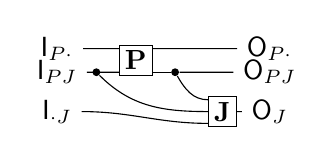
\begin{tikzpicture}[baseline={([yshift=-.2ex]current bounding box.center)}]
        \path (0,0) node (Y) {$\RV{I}_{P\cdot}$}
        + (0,-0.3) node (Q) {$\RV{I}_{PJ}$}
        + (0,-0.8) node (R) {$\RV{I}_{\cdot J}$}
        ++ (0.5,-0.3) node[copymap] (copy0) {}
        ++ (0.5,0.15) node[kernel] (K) {$\kernel{P}$}
        ++ (0.5,-0.15) node[copymap] (copy1) {}
        ++ (0.6,-0.5) node[kernel] (L) {$\kernel{J}$}
        ++ (0.6, 0.8) node (Z) {$\RV{O}_{P\cdot}$}
        + (0,-0.3) node (X) {$\RV{O}_{PJ}$}
        + (0,-0.8) node (W) {$\RV{O}_J$};
        \draw (Y) -- ($(K.west) + (0,0.15)$) (Q) -- ($(K.west) + (0,-0.15)$);
        \draw (copy0) to [out=-45,in=180] ($(L.west) + (0,0)$) (copy1) to [out=-60,in=180] ($(L.west) + (0,0.15)$);
        \draw (R) to [out=0,in=180] ($(L.west) + (0,-0.15)$);
        \draw ($(K.east) + (0,-0.15)$) to (copy1);
        \draw ($(K.east) + (0,0.15)$) -- (Z) (copy1) to [out=0,in=180] (X) (L) -- (W);
    \end{tikzpicture}\\
    &= 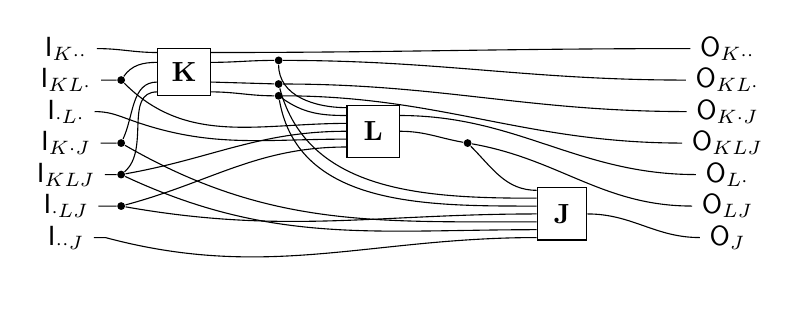
\begin{tikzpicture}[baseline={([yshift=-.2ex]current bounding box.center)}] \path (0,0) node (IKdd) {$\RV{I}_{K\cdot\cdot}$}
        + (0,-0.4) node (IKLd) {$\RV{I}_{KL\cdot}$}
        + (0,-0.8) node (IdLd) {$\RV{I}_{\cdot L \cdot}$}
        + (0,-1.2) node (IKdJ) {$\RV{I}_{K\cdot J}$}
        + (0,-1.6) node (IKLJ) {$\RV{I}_{KLJ}$}
        + (0,-2) node (IdLJ) {$\RV{I}_{\cdot LJ}$}
        + (0,-2.4) node (IddJ) {$\RV{I}_{\cdot\cdot J}$}
        + (0.7,-0.4) node[copymap] (copyKL) {}
        + (0.7,-1.2) node[copymap] (copyKJ) {}
        + (0.7,-1.6) node[copymap] (copyKLJ) {}
        + (0.7,-2) node[copymap] (copyLJ) {}
        ++ (1.5,-0.3) node[kernel,inner sep=5pt] (K) {$\kernel{K}$}
        ++ (1.2,0.15) node[copymap] (copyOKL) {}
        +  (0,-0.3) node[copymap] (copyOKJ) {}
        + (0,-0.45) node[copymap] (copyOKLJ) {}
        ++ (1.2,-0.9) node[kernel,inner sep=6pt] (L) {$\kernel{L}$}
        ++ (1.2,-0.15) node[copymap] (copyOLJ) {}
        ++ (1.2,-0.9) node[kernel,inner sep=6pt] (J) {$\kernel{J}$}
        ++ (2.1, 2.1) node (OKdd) {$\RV{O}_{K\cdot\cdot}$}
        + (0,-0.4) node (OKLd) {$\RV{O}_{KL\cdot}$}
        + (0,-0.8) node (OKdJ) {$\RV{O}_{K\cdot J}$}
        + (0,-1.2) node (OKLJ) {$\RV{O}_{KLJ}$}
        + (0,-1.6) node (OLd) {$\RV{O}_{L\cdot}$}
        + (0,-2) node (OLJ) {$\RV{O}_{LJ}$}
        + (0,-2.4) node (OJ) {$\RV{O}_{J}$};
        \draw (IKdd) to [out=0,in=180] ($(K.west) + (0,0.25)$) ($(K.east) + (0,0.25)$) to [out=0,in=180] (OKdd);
        \draw (IKLd) -- (copyKL) to [out=-45,in=180] ($(L.west) + (0,0.1)$) (copyKL) to [out=55,in=180] ($(K.west) + (0,0.125)$)
        ($(K.east)+(0,0.125)$) to [out=0,in=180] (copyOKL) to [out=-90,in=180] ($(L.west) + (0,0.3)$)
        (copyOKL) to [out=0,in=180] (OKLd);
        \draw (IKLJ) to [out=0,in=180] (copyKLJ) to [out=40,in=180] ($(K.west) + (0,-0.25)$) 
        (copyKLJ) to [out=10,in=180] ($(L.west) + (0,0)$)
        (copyKLJ) to [out=-25,in=180] ($(J.west) + (0,-0.2)$);
        \draw (IKdJ) to [out=0,in=180] (copyKJ) to [out=65,in=180] ($(K.west) + (0,-0.125)$)
        (copyKJ) to [out=-30,in=180] ($(J.west) + (0,-0.1)$);
        \draw (IdLd) to [out=0,in=160] ($(IdLd)+(0.8,-0.1)$) to [out=-20,in=180] ($(L.west)+(0,-0.1)$);
        \draw (IdLJ) to [out=0,in=180] (copyLJ) to[out=15,in=180] ($(L.west)+(0,-0.2)$)
        (copyLJ) to [out=-10,in=180] ($(J.west) + (0,0.)$);
        \draw (IddJ) to [out=0,in=180] ($(IddJ)+ (0.5,0)$) to [out=-15,in=180] ($(J.west) + (0,-0.3)$);
        \draw ($(K.east)+(0,-0.125)$) to (copyOKJ) to [out=-75,in=180] ($(J.west) + (0,0.2)$)
        (copyOKJ) to [out=0,in=180] (OKdJ)
        (copyOKLJ) to [out=-80,in=180] ($(J.west) + (0,0.1)$);
        \draw ($(K.east) + (0,-0.25)$) to [out=0,in=180] (copyOKLJ) to [out=0,in=180] (OKLJ)
        (copyOKLJ) to [out=-35,in=180] ($(L.west) + (0,0.2)$);
        \draw ($(L.east) + (0,0.2)$) to [out=0,in=180] (OLd)
        ($(L.east) + (0,0)$) to [out=0,in=170] (copyOLJ) to [out=-10,in=180] (OLJ)
        (copyOLJ) to [out=-45,in=180] ($(J.west) + (0,0.3)$);
        \draw (J) to [out=0,in=180] (OJ);
    \end{tikzpicture}\\
    &\overset{perm}{=} 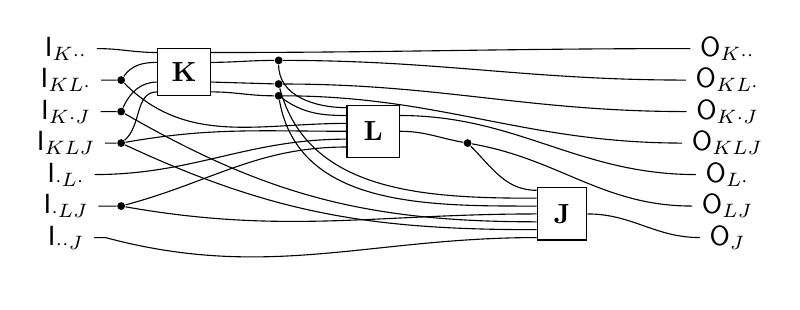
\begin{tikzpicture}[baseline={([yshift=-.2ex]current bounding box.center)}] \path (0,0) node (IKdd) {$\RV{I}_{K\cdot\cdot}$}
        + (0,-0.4) node (IKLd) {$\RV{I}_{KL\cdot}$}
        + (0,-0.8) node (IKdJ) {$\RV{I}_{K\cdot J}$}
        + (0,-1.2) node (IKLJ) {$\RV{I}_{KLJ}$}
        + (0,-1.6) node (IdLd) {$\RV{I}_{\cdot L \cdot}$}
        + (0,-2) node (IdLJ) {$\RV{I}_{\cdot LJ}$}
        + (0,-2.4) node (IddJ) {$\RV{I}_{\cdot\cdot J}$}
        + (0.7,-0.4) node[copymap] (copyKL) {}
        + (0.7,-.8) node[copymap] (copyKJ) {}
        + (0.7,-1.2) node[copymap] (copyKLJ) {}
        + (0.7,-2) node[copymap] (copyLJ) {}
        ++ (1.5,-0.3) node[kernel,inner sep=5pt] (K) {$\kernel{K}$}
        ++ (1.2,0.15) node[copymap] (copyOKL) {}
        +  (0,-0.3) node[copymap] (copyOKJ) {}
        + (0,-0.45) node[copymap] (copyOKLJ) {}
        ++ (1.2,-0.9) node[kernel,inner sep=6pt] (L) {$\kernel{L}$}
        ++ (1.2,-0.15) node[copymap] (copyOLJ) {}
        ++ (1.2,-0.9) node[kernel,inner sep=6pt] (J) {$\kernel{J}$}
        ++ (2.1, 2.1) node (OKdd) {$\RV{O}_{K\cdot\cdot}$}
        + (0,-0.4) node (OKLd) {$\RV{O}_{KL\cdot}$}
        + (0,-0.8) node (OKdJ) {$\RV{O}_{K\cdot J}$}
        + (0,-1.2) node (OKLJ) {$\RV{O}_{KLJ}$}
        + (0,-1.6) node (OLd) {$\RV{O}_{L\cdot}$}
        + (0,-2) node (OLJ) {$\RV{O}_{LJ}$}
        + (0,-2.4) node (OJ) {$\RV{O}_{J}$};
        \draw (IKdd) to [out=0,in=180] ($(K.west) + (0,0.25)$) ($(K.east) + (0,0.25)$) to [out=0,in=180] (OKdd);
        \draw (IKLd) -- (copyKL) to [out=-45,in=180] ($(L.west) + (0,0.1)$) (copyKL) to [out=55,in=180] ($(K.west) + (0,0.125)$)
        ($(K.east)+(0,0.125)$) to [out=0,in=180] (copyOKL) to [out=-90,in=180] ($(L.west) + (0,0.3)$)
        (copyOKL) to [out=0,in=180] (OKLd);
        \draw (IKLJ) to [out=0,in=180] (copyKLJ) to [out=40,in=180] ($(K.west) + (0,-0.25)$) 
        (copyKLJ) to [out=10,in=180] ($(L.west) + (0,0)$)
        (copyKLJ) to [out=-25,in=180] ($(J.west) + (0,-0.2)$);
        \draw (IKdJ) to [out=0,in=180] (copyKJ) to [out=65,in=180] ($(K.west) + (0,-0.125)$)
        (copyKJ) to [out=-30,in=180] ($(J.west) + (0,-0.1)$);
        \draw (IdLd) to [out=0,in=180] ($(L.west)+(0,-0.1)$);
        \draw (IdLJ) to [out=0,in=180] (copyLJ) to[out=15,in=180] ($(L.west)+(0,-0.2)$)
        (copyLJ) to [out=-10,in=180] ($(J.west) + (0,0.)$);
        \draw (IddJ) to [out=0,in=180] ($(IddJ)+ (0.5,0)$) to [out=-15,in=180] ($(J.west) + (0,-0.3)$);
        \draw ($(K.east)+(0,-0.125)$) to (copyOKJ) to [out=-75,in=180] ($(J.west) + (0,0.2)$)
        (copyOKJ) to [out=0,in=180] (OKdJ)
        (copyOKLJ) to [out=-80,in=180] ($(J.west) + (0,0.1)$);
        \draw ($(K.east) + (0,-0.25)$) to [out=0,in=180] (copyOKLJ) to [out=0,in=180] (OKLJ)
        (copyOKLJ) to [out=-35,in=180] ($(L.west) + (0,0.2)$);
        \draw ($(L.east) + (0,0.2)$) to [out=0,in=180] (OLd)
        ($(L.east) + (0,0)$) to [out=0,in=170] (copyOLJ) to [out=-10,in=180] (OLJ)
        (copyOLJ) to [out=-45,in=180] ($(J.west) + (0,0.3)$);
        \draw (J) to [out=0,in=180] (OJ);
    \end{tikzpicture}\\
    &= 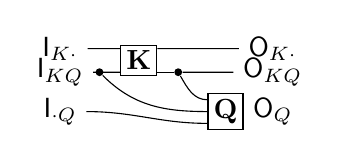
\begin{tikzpicture}[baseline={([yshift=-.2ex]current bounding box.center)}]
        \path (0,0) node (Y) {$\RV{I}_{K\cdot}$}
        + (0,-0.3) node (Q) {$\RV{I}_{KQ}$}
        + (0,-0.8) node (R) {$\RV{I}_{\cdot Q}$}
        ++ (0.5,-0.3) node[copymap] (copy0) {}
        ++ (0.5,0.15) node[kernel] (K) {$\kernel{K}$}
        ++ (0.5,-0.15) node[copymap] (copy1) {}
        ++ (0.6,-0.5) node[kernel] (L) {$\kernel{Q}$}
        ++ (0.6, 0.8) node (Z) {$\RV{O}_{K\cdot}$}
        + (0,-0.3) node (X) {$\RV{O}_{KQ}$}
        + (0,-0.8) node (W) {$\RV{O}_Q$};
        \draw (Y) -- ($(K.west) + (0,0.15)$) (Q) -- ($(K.west) + (0,-0.15)$);
        \draw (copy0) to [out=-45,in=180] ($(L.west) + (0,0)$) (copy1) to [out=-60,in=180] ($(L.west) + (0,0.15)$);
        \draw (R) to [out=0,in=180] ($(L.west) + (0,-0.15)$);
        \draw ($(K.east) + (0,-0.15)$) to (copy1);
        \draw ($(K.east) + (0,0.15)$) -- (Z) (copy1) to [out=0,in=180] (X) (L) -- (W);
    \end{tikzpicture}\\
    &= \kernel{K}\rightrightarrows (\kernel{L}\rightrightarrows \kernel{J})
\end{align}

\section{Appendix: String Diagram Examples}

Recall the definition of \emph{connection}:
\begin{definition}[Connection]
\begin{align}
    \kernel{K}\rightrightarrows \kernel{L} &:=  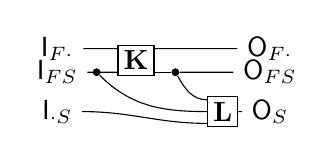
\begin{tikzpicture}[baseline={([yshift=-.2ex]current bounding box.center)}]
        \path (0,0) node (Y) {$\RV{I}_{F\cdot}$}
        + (0,-0.3) node (Q) {$\RV{I}_{FS}$}
        + (0,-0.8) node (R) {$\RV{I}_{\cdot S}$}
        ++ (0.5,-0.3) node[copymap] (copy0) {}
        ++ (0.5,0.15) node[kernel] (K) {$\kernel{K}$}
        ++ (0.5,-0.15) node[copymap] (copy1) {}
        ++ (0.6,-0.5) node[kernel] (L) {$\kernel{L}$}
        ++ (0.6, 0.8) node (Z) {$\RV{O}_{F\cdot}$}
        + (0,-0.3) node (X) {$\RV{O}_{FS}$}
        + (0,-0.8) node (W) {$\RV{O}_S$};
        \draw (Y) -- ($(K.west) + (0,0.15)$) (Q) -- ($(K.west) + (0,-0.15)$);
        \draw (copy0) to [out=-45,in=180] ($(L.west) + (0,0)$) (copy1) to [out=-60,in=180] ($(L.west) + (0,0.15)$);
        \draw (R) to [out=0,in=180] ($(L.west) + (0,-0.15)$);
        \draw ($(K.east) + (0,-0.15)$) to (copy1);
        \draw ($(K.east) + (0,0.15)$) -- (Z) (copy1) to [out=0,in=180] (X) (L) -- (W);
    \end{tikzpicture}\label{eq:extn_definition1}\\
    &:= \kernel{J}\\
    \kernel{J}_{yqr}^{zxw} &= \kernel{K}_{yq}^{zx} \kernel{L}_{xqr}^{w}\label{eq:extn_definition2}
\end{align}
\end{definition}

Equation \ref{eq:extn_definition1} can be broken down to the product of four Markov kernels, each of which is itself a tensor product of a number of other Markov kernels:
\begin{align}
    (\kernel{J},(\RV{I}_{F\cdot},\RV{I}_{FS},\RV{I}_{\cdot S}), (\RV{O}_{F\cdot},\RV{O}_{FS},\RV{O}_S)) &= \left[ 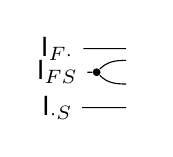
\begin{tikzpicture}[baseline={([yshift=-.5ex]current bounding box.center)}]
        \path (0,0) node (Y) {$\RV{I}_{F\cdot}$}
        + (0,-0.3) node (Q) {$\RV{I}_{FS}$}
        + (0,-0.75) node (R) {$\RV{I}_{\cdot S}$}
        ++ (0.5,-0.3) node[copymap] (copy1) {}
        ++ (0.5,0.3) node (Z) {}
        ++ (0,-0.15) node (Q1) {}
        ++ (0,-0.3) node (Q2) {}
        ++ (0,-0.3) node (R2) {};
        \draw (Y) -- (Z) (Q) -- (copy1) to [out=45,in=180] (Q1);
        \draw (copy1) to [out=-45,in=180] (Q2);
        \draw (R) -- (R2); \end{tikzpicture}\right]
        \left[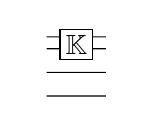
\begin{tikzpicture}[baseline={([yshift=-.5ex]current bounding box.center)}]
        \path (0,0)  node (Z) {}
        ++ (0,-0.15) node (Q1) {}
        ++ (0,-0.3) node (Q2) {}
        ++ (0,-0.3) node (R) {}
        ++ (0.5,0.65) node[kernel] (K) {$\model{K}$}
        ++ (0.5,0.1) node (Z1) {}
        +  (0,-0.15) node (W) {}
        + (0,-0.45) node (Q3) {}
        + (0,-0.75) node (R2) {};
        \draw (Z) -- ($(K.west) + (0,0.1)$) (Q1) -- ($(K.west) + (0,-0.05)$);
        \draw (Q2) -- (Q3) (R) -- (R2) ($(K.east) + (0,0.1)$) -- (Z1); 
        \draw ($(K.east) + (0,-0.05)$) -- (W);\end{tikzpicture}\right] 
        \left[ 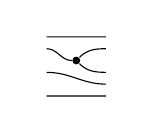
\begin{tikzpicture}[baseline={([yshift=-.5ex]current bounding box.center)}]
        \path (0,0) node (Z) {}
        + (0,-0.15) node (X) {}
        + (0,-0.45) node (Q) {}
        + (0,-0.75) node (R) {}
        ++ (0.5,-0.3) node[copymap] (copy1) {}
        ++ (0.5,0.3) node (Z1) {}
        ++ (0,-0.15) node (X1) {}
        ++ (0,-0.3) node (X2) {}
        ++ (0,-0.15) node (Q2) {}
        ++ (0,-0.15) node (R2) {};
        \draw (Z) -- (Z1) (X) to [out=0,in=180] (copy1) to [out=45,in=180] (X1);
        \draw (copy1) to [out=-45,in=180] (X2);
        \draw (Q) to [out=0,in=180] (Q2);
        \draw (R) -- (R2); \end{tikzpicture}\right]
        \left[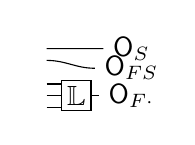
\begin{tikzpicture}[baseline={([yshift=-.5ex]current bounding box.center)}]
        \path (0,0) node (Z) {}
        ++ (0,-0.15) node (X1) {}
        ++ (0,-0.3) node (X2) {}
        ++ (0,-0.15) node (Q) {}
        ++ (0,-0.15) node (R) {}
        ++ (0.5,0.15) node[kernel] (L) {$\model{L}$}
        ++ (0.7,0) node (W) {$\RV{O}_{F\cdot}$}
        ++ (0,0.35) node (X3) {$\RV{O}_{FS}$}
        ++ (0,0.25) node (Z1) {$\RV{O}_S$};
        \draw (X1) to [out=0,in=180] (X3) (Z) -- (Z1);
        \draw (X2) to [out=0,in=180] ($(L.west) + (0,0.15)$);
        \draw (Q) to [out=0,in=180] ($(L.west) + (0,0)$);
        \draw (R) to [out=0,in=180] ($(L.west) + (0,-0.15)$);
        \draw (L) -- (W);\end{tikzpicture}\right]\\
\end{align}

\section{Markov variable maps and variables form a Markov category}\label{sec:app_mcat}

In the following, given \emph{arbitrary measurable sets} $(X,\sigalg{X})$ and $(Y,\sigalg{Y})$, a Markov kernel is a function $\kernel{K}:X\times\sigalg{Y}\to [0,1]$ such that

\begin{itemize}
    \item For every $A\in \sigalg{Y}$, the function $x\mapsto \kernel{K}(x,A)$ is $\sigalg{X}$-measurable
    \item For every $x\in X$, the function $A\mapsto \kernel{K}(x,A)$ is a probability measure on $(Y,\sigalg{Y})$
\end{itemize}

Note that this is a more general definition than the one used in the main paper; the version in the main paper is the restriction of this definition to finite sets.

The \emph{delta function} $\delta:X\to\Delta(\sigalg{X})$ is the Markov kernel defined by
\begin{align}
    \delta(x,A) = \begin{cases}
        1 & x\in A\\
        0 & \text{otherwise}
    \end{cases}
\end{align}

\citet{fritz_synthetic_2020} defines Markov categories in the following way:

\begin{definition}
A Markov category $C$ is a symmetric monoidal category in which every object $X \in C$ is equipped with a commutative comonoid structure given by a comultiplication $\text{copy}_X : X\to X\otimes X$ and a counit $\text{del}_X : X \to I$, depicted in string diagrams as
\begin{align}
    \text{del}_X&:=\begin{tikzpicture}[baseline={([yshift=-.5ex]current bounding box.center)}]
    \path (0,0) ++ (1,0) node (B) {};
    \draw[-{Rays[n=8]}] (A) -- (B);
\end{tikzpicture}
    \text{copy}_X&:=\begin{tikzpicture}[baseline={([yshift=-.5ex]current bounding box.center)}]
    \path (0,0) node (A) {} 
    ++ (0.5,0) node[copymap] (copy0) {}
    ++ (0.5,0.15) node (B) {}
    + (0,-0.3) node (C) {};
    \draw (A) -- (copy0) to [out=45,in=180] (B) (copy0) to [out=-45, in=180] (C);
\end{tikzpicture}
\end{align}
and satisfying the commutative comonoid equations
\begin{align}
    \tikzfig{ccom_lhs} = \tikzfig{ccom_rhs}\label{eq:ccom_1}
\end{align}
\begin{align}
    \tikzfig{ccom2_lhs} = \tikzfig{ccom2_mhs} = \tikzfig{ccom2_rhs}
\end{align}
\begin{align}
    \tikzfig{ccom3_lhs} = \tikzfig{ccom3_rhs}
\end{align}
as well as compatibility with the monoidal structure
\begin{align}
    \tikzfig{mstruct1_lhs} &= \tikzfig{mstruct1_rhs}\\
    \tikzfig{mstruct2_lhs} &= \tikzfig{mstruct2_rhs}
\end{align}
and the naturality of \emph{del}, which means that
\begin{align}
    \tikzfig{naturality_lhs} &= \tikzfig{naturality_rhs}\label{eq:nat}
\end{align}
for every morphism $f$.
\end{definition}

The category of labeled Markov kernels is the category consisting of labeled measurable sets as objects and labeled Markov kernels as morphisms. Given $\kernel{K}:\RV{X}\to \Delta(\RV{Y})$ and $\kernel{L}:\RV{Y}\to \Delta(\RV{Z})$, sequential composition is given by

\begin{align}
    \kernel{K}\kernel{L}:\RV{X}\to \Delta(\RV{Z})\\
    \text{defined by } (\kernel{KL})(x,A) = \int_Y \kernel{L}(y,A)\kernel{K}(x,dy)
\end{align}

For $\kernel{K}:\RV{X}\to \Delta(\RV{Y})$ and $\kernel{L}:\RV{W}\to\Delta(\RV{Z})$, parallel composition is given by

\begin{align}
    \kernel{K}\otimes\kernel{L}: (\RV{X},\RV{W}) &\to \Delta(\RV{Y},\RV{Z})\\
    \text{defined by } \kernel{K}\otimes\kernel{L}(x,w,A\times B) = \kernel{K}(x,A)\kernel{L}(w,B)
\end{align}

The identity map is

\begin{align}
    \text{Id}_{\RV{X}}: \RV{X}&\to\Delta(\RV{X})\\
    \text{defined by} (\text{Id}_X) (x,A) &= \delta(x,A)
\end{align}

We take an arbitrary single element labeled set $I=(*,\{*\})$ to be the unit, which we note satisfies $I\otimes X=X\otimes I=X$ by Lemma \ref{lem:se_id}.

The swap map is given by

\begin{align}
    \text{swap}_{\RV{X},\RV{Y}}: (\RV{X},\RV{Y})&\to \Delta(\RV{Y},\RV{X})\\
    \text{defined by} (\text{swap}_{\RV{X},\RV{Y}})(x,y,A\times B) &= \delta(x,B)\delta(y,A)
\end{align}

And we use the standard associativity isomorphisms for Cartesian products such that $(A\times B)\times C\cong A\times (B\times C)$, which in turn implies $(\RV{X},(\RV{Y},\RV{Z}))\cong ((\RV{X},\RV{Y}),\RV{Z})$.

The copy map is given by

\begin{align}
    \text{copy}_{\RV{X}}: \RV{X}&\to \Delta(\RV{X},\RV{X})\\
    \text{defined by} (\text{copy}_X)(x,A\times B) &= \delta_x(A)\delta_x(B)
\end{align}

and the erase map by

\begin{align}
    \text{del}_{\RV{X}}: \RV{X}&\to \Delta(*)\\
    \text{defined by} (\text{del}_X)(x,A) &= \delta(*,A)\\
\end{align}

Note that the category formed by taking the underlying unlabeled sets and the underlying unlabeled morphisms is identical to the category of measurable sets and Markov kernels described in \citet{fong_causal_2013,cho_disintegration_2019,fritz_synthetic_2020}.

\begin{theorem}[The category of labeled Markov kernels and labeled measurable sets is a Markov category]
The category described above is a Markov category.
\end{theorem}

\begin{proof}

\todo[inline]{I'm not sure how to formally argue that it is monoidal and symmetric as the relevant texts I've checked all gloss over the functors with respect to which the relevant isomorphisms should be natural, but labels with products were intentionally made to act just like sets with cartesian products which are symmetric monoidal}

Equations \ref{eq:ccom_1} to \ref{eq:nat} are known to be satisfied for the underlying unlabeled Markov kernels. We need to show is that they hold given our stricter criterion of labeled Markov kernel equality; that the underlying kernels \emph{and the label sets} match. It is sufficient to check the label sets only.



\end{proof}
% \input{chapter_3_twoplayer_statistical_models}
% \input{chapter_4_statistical_decision_theory}
% \input{chapter_5_interventions_counterfactuals}
% \input{chapter_6_imitability_inference}
% \input{chapter_7_godscomputer}

\bibliographystyle{plainnat}
\bibliography{references}

\appendix
\newpage
\section*{Appendix:}

% \input{appendix_AIstats}

\end{document}
